\documentclass[pdflatex,11pt]{aghdpl}
%\documentclass[pdflatex,11pt,openright,b5paper]{pl_book}
% \documentclass{aghdpl}               % przy kompilacji programem latex
% \documentclass[pdflatex,en]{aghdpl}  % praca w~języku angielskim
\usepackage{hyphenat}
\usepackage{url}
\usepackage[T1]{fontenc}
\usepackage{natbib}
\usepackage[polish]{babel}
\usepackage[utf8]{inputenc}
\usepackage{wrapfig}
\usepackage{graphicx}
\usepackage{subcaption}
\usepackage[font={small}]{caption}
\usepackage{float}
\usepackage{amsmath}
\usepackage{amsfonts}
\usepackage[outercaption]{sidecap}    
\usepackage{textcomp}

\usepackage{titlesec}
\titleclass{\chapter}{top}

\setcitestyle{square}


\usepackage{nomencl}
\makenomenclature

% dodatkowe pakiety
\usepackage{enumerate}
\usepackage{listings}
\lstloadlanguages{TeX}

\lstset{
  literate={ą}{{\k{a}}}1
           {ć}{{\'c}}1
           {ę}{{\k{e}}}1
           {ó}{{\'o}}1
           {ń}{{\'n}}1
           {ł}{{\l{}}}1
           {ś}{{\'s}}1
           {ź}{{\'z}}1
           {ż}{{\.z}}1
           {Ą}{{\k{A}}}1
           {Ć}{{\'C}}1
           {Ę}{{\k{E}}}1
           {Ó}{{\'O}}1
           {Ń}{{\'N}}1
           {Ł}{{\L{}}}1
           {Ś}{{\'S}}1
           {Ź}{{\'Z}}1
           {Ż}{{\.Z}}1
}

%---------------------------------------------------------------------------

\author{Marcin Stolarek}
\shortauthor{M. Stolarek}

%\titlePL{Elementy dyfrakcyjne, refracyjne i~absorpcyjne oparte na podfalowych periodycznych strukturach metalicznych}
\titlePL{Elementy dyfrakcyjne, refrakcyjne i~absorpcyjne oparte na podfalowych periodycznych strukturach metalicznych}
\titleEN{Diffractive, refractive and absorptive optical elements based on periodic sub-wavelength metallic structures}

%\shorttitle{Elementy dyfrakcyjne, refracyjne i~absorpcyjne oparte na podfalowych periodycznych strukturach metalicznych} % skrócona wersja tytułu jeśli jest bardzo długi
\shorttitlePL{Elementy dyfrakcyjne, refrakcyjne i~absorpcyjne oparte na podfalowych periodycznych strukturach metalicznych} % skrócona wersja tytułu jeśli jest bardzo długi
\shorttitleEN{Diffractive, refractive and absorptive optical elements based on periodic sub-wavelength metallic structures}

%\thesistype{Rozprawa doktorska}
\thesistypePL{Rozprawa doktorska}
\thesistypeEN{Phd in physics}

%\supervisor{dr hab. Rafał Kotyński}
\supervisorPL{dr hab. Rafał Kotyński}
\supervisorEN{Rafał Kotyński Ph.D}

\date{2016}

\departmentPL{Zakład Optyki Informacyjnej}
\departmentEN{Information Optics Department}

\facultyPL{Wydział Fizyki}
\facultyEN{Faculty of Physics}



\setlength{\cftsecnumwidth}{10mm}

%---------------------------------------------------------------------------

\begin{document}


\frontmatter

\titlepages

\section*{Podziękowania}
Powstanie niniejszej rozprawy doktorskiej nie byłoby możliwe bez opieki dra~hab.~Rafała Kotyńskiego, który przez cały czas moich studiów doktoranckich i powstawania tej pracy sprawował nade mną opiekę merytoryczną. Zarówno za to, jak i za wiele, często krótkich, wymian zdań na temat stanu i sensu uprawiania współczesnej nauki, które czasem ułatwiały mi rozładowanie negatywnych emocji związanych z pracą fizyka, serdecznie Ci, Rafale dziękuję.

Szczególne podziękowania składam również prof.~Tomaszowi Szoplikowi. Sprawował On nade mną opiekę promotorską przez pierwsze dwa lata moich studiów doktoranckich, a przez cały czas ich trwania służył radą zarówno w kwestiach merytorycznych, jak i organizacyjnych. To również za jego namową nie przerwałem studiów, co było warunkiem koniecznym powstania tej pracy.

Dziękuję również koleżankom i kolegom, z którymi miałem okazję pracować nad różnymi projektami. Specjalne podziękowania należą się Ani Pastuszczak, która nie tylko współpracowała ze mną w trakcie studiów, lecz także podjeła się również przeczytania tej pracy w wersji rozwojowej. Bez jej komentarzy niniejsza rozprawa okazałaby się dla czytelnika mniej przyjazna.

Dziękuję również swoim rodzicom, dzięki którym mogłem podjąć studia na Wydziale Fizyki. Jestem wdzięczny zwłaszcza za wsparcie, które od Was otrzymałem w trakcie trudnych pierwszych lat studiów.  

Osobne podziękowania kieruję do Karolci, która była ze mną przez cały, nie zawsze łatwy, czas powstawania tej pracy.
\clearpage

\tableofcontents
\clearpage

\mainmatter



\section{State of the art}
\section{Cele i tezy pracy}
\section{Podział pracy}












\section{Metody numeryczne}
\subsection{Metody  macierzowe}
\subsection{FDTD}
Przykladowe rozwiązania: fala zanikajaca, plazmon, fala propagujaca?
\section{Systemy liniowe niezmiennicze.}
Celem ninejszego podrozdziału jest zdefiniowanie pojęcia systemów liniowych, które w~niniejszej pracy znajduje zastosowanie w~analizie zjawisk obrazowania. W ogólności, przez systemem rozumiemy odpowiedniość pomiędzy zestawem funkcji wejściowych, a zestawem funkcji wyjściowych. W przypadku sieci elektrycznych funkcjami wejściowymi jak i~wyjściowymi mogą być zależności napięcia i~natężenia prądu elektrycznego od czasu. Jeżeli ograniczymy opis do systemów deterministycznych, określonemu zestawowi funkcji wejściowych musi odpowiadać dokładnie jeden układ funkcji wyjściowych. Wyjście układu nie musi jednak pozwalać na jednoznaczną identyfikację wejścia, w~szczególności dla wielu stanów wejścia system może nie odpowiadać żadnym wyjściem.

\label{art:lsi}

Matematyczną reprezentacją opisanego systemu, jest operator $S\{\}$, który działając na zbiór funkcji wejściowych $g_i$ tworzy funkcje wyjściowe $f_i$:
\begin{equation}
f_i(\vec{x})=S\{g_i(\vec{x})\}.
\label{eq:system}
\end{equation} 
Warunkiem liniowości systemu opisywanego operatorem $S\{\}$ jest liniowość samego operatora $S\{\}$, która wymaga spełnienia zasady superpozycji matematycznie wyrażonej przez poniższe równanie
\begin{equation}
S\{\alpha p(\vec{x}) + \beta q(\vec{x})\} = \alpha S\{p(\vec{x})\} + \beta S\{q(\vec{x})\},
\label{eq:lin-system}
\end{equation}
spełnione dla dowolnych zespolonych skalarów $\alpha$ i~$\beta$, oraz dowolnych funkcji $p(\vec{x})$ i~$q(\vec{x})$. Zgodnie z~powyższym równaniem, odpowiedź systemu możemy przedstawić jako sumę odpowiedzi na funkcje składowe na które rozłożyliśmy wejście układu. W przypadku zjawisk elektromagnetycznych zasada superpozycji spełniona jest dla amplitud pól elektromagnetycznych w~przypadku promieniowania koherentnego, oraz dla natężeń pól w~przypadku promieniowania nie koherentnego. Do rozkładu funkcji wejściowej na elementarne składowe posłużymy się własnością filtracji delty Diraca
\begin{equation}
g(\vec{x})=\int_{-\infty}^{+\infty} g(\vec{\eta}) \delta(x-\eta) d \vec{\eta}.
\label{eq:dirac-shifting}
\end{equation}
Poszukując funkcji wyjściowej dla układu $S\{\}$ odpowiadającej funkcji wejściowej $g(x)$, wykonujemy podstawienie równania \ref{eq:dirac-shifting} do równania \ref{eq:system} 
\begin{equation}
f(\vec{x})=S \{\int_{-\infty}^{+\infty} g(\vec{\eta}) \delta(\vec{x}-\vec{\eta}) d \vec{\eta} \}.
\label{eq:dirac-shift2}
\end{equation}
Ponieważ funkcja $g(\vec{\eta})$ nie zależy od zmiennych $\vec{x}$, możemy traktować ją jako wagę i~korzystając z~własności superpozycji \ref{eq:lin-system} włączyć operator $S{}$ pod znak całki
\begin{equation}
f(\vec{x})=\int_{-\infty}^{+\infty} g(\vec{\eta})  S\{\delta(\vec{x}-\vec{\eta}) d \vec{\eta} \},
\label{eq:dirac-shift3}
\end{equation}
dla uproszczenia zapisu powyższego równania wprowadzimy funkcję
\begin{equation}
h(\vec{x},\vec{\eta}):=S\{\delta(\vec{x}-\vec{\eta})\}.
\label{eq:imp-resp}
\end{equation}
Powyższa funkcja nazywana jest funkcją odpowiedz impulsowej (ang. impluse response), w~optyce zazwyczaj określa się ją mianem funkcji rozmycia punktu (ang. point-spread function). Korzystając z~wprowadzonego oznaczenia możemy do równania \ref{eq:dirac-shift3}  podstawić definicję \ref{eq:imp-resp}, otrzymując jedną z~podstawowych formuł stosowanych do opisu systemów liniowych, tzw. całkę superpozycji:
\begin{equation}
f(\vec{x})=\int_{-\infty}^{+\infty} g(\vec{\eta})  h(\vec{x},\vec{\eta}) d \vec{\eta} .
\label{eq:sup-int}
\end{equation}
Powyższe równanie wskazuje, że dla opisania odpowiedzi systemu na dowolną funkcję wejściową, niezbędna jest jedynie znajomość funkcji odpowiedzi impulsowej układu. W ogólnym przypadku, funkcja odpowiedzi musi być zdefiniowana dla wszystkich punktowych wzbudzeń w~płaszczyźnie wejściowej. Przykładem analizowanego układu może być np. soczewka oświetlana promieniowaniem niekoherentnym, dla której niezbędnym zestawem informacji potrzebnym do obliczenia natężenia światła w~płaszczyźnie obrazu jest znajomość funkcji odpowiedzi dla wszystkich źródeł punktowych znajdujących się w~płaszczyźnie przedmiotu. 

Szczególne znaczenie dla niniejszej pracy ma kolejna, często spotykana w~zastosowaniach własność układów liniowych określana jako niezmienniczość. W ogólności, może być to np. niezmienniczość systemu elektrycznego w~czasie. 
%Rozumiana jako zależność funkcji odpowiedzi impulsowej $h(t,\tau)$ (gdzie $t$ jest czasem, w~którym poszukiwana jest odpowiedź na impuls elektryczny mający miejsce w~czasie $\tau$) jedynie od różnicy $t-\tau$. Dla układów elektrycznych taka własność jest zazwyczaj spełniona, ponieważ oporniki, kondensatory i~indukcyjności z~których są zbudowane zazwyczaj nie zmieniają swoich własności w~czasie eksperymentów.

Dla układu obrazującego istotną rolę odgrywa izoplanatyczność - niezmienniczość ze względu na przesunięcia, w~wyniku której, funkcja odpowiedzi impulsowej zależy jedynie od odległości pomiędzy położeniem wzbudzenia, a położeniem obrazu
\begin{equation}
h(\vec{x},\vec{\eta})=h(\vec{x}-\vec{\eta}).
\label{eq:shif-inv}
\end{equation}
Powyższa własność zastosowana do układów obrazujących jest więc równoważna stwierdzeniu, że zmiana położenia przedmiotu wpływa jedynie na zmianę położenia jego obrazu. W przypadku niemal wszystkich realnych układów optycznych własność ta nie jest spełniona w~całej przestrzeni położeń, zazwyczaj można jednak obszar podzielić na podobszary, w~których zastosowanie będą miały odpowiednie funkcje $h_i$, natomiast w~ramach pojedynczego podobszaru z~dobrym przybliżeniem stosować można założenie o~izoplanatyczności systemu. Szczególnym przypadkiem obszaru często wykorzystywanego w~analizie obrazowania przez klasyczne elementy optyczne jest otoczenie osi układu, w~stosunku do którego stosuje się omawiane przybliżenie.

Podstawiając równanie (\ref{eq:shif-inv} )do wzoru (\ref{eq:sup-int}) otrzymujemy
\begin{equation}
f(\vec{x})=\int_{-\infty}^{+\infty} g(\vec{\eta})  h(\vec{x}-\vec{\eta}) d \vec{\eta} = g \ast h.
\label{eq:splot}
\end{equation}
W powyższym równaniu $\ast$ oznacza operację splotu. Dzięki sprowadzeniu całki superpozycji dla układów liniowych niezmienniczych ze względu na przesunięcia (ang. LSI - linear shift-invariant) do tej szczególnej postaci, możemy do analizy układów LSI wykorzystać kolejne twierdzenia analizy matematycznej. Ważne znaczenie odgrywa twierdzenie o~splocie, będącego jedną z~podstawowych własności transformaty Fouriera. Zapiszemy powyższe równanie jako
\begin{equation}
F\{f(\vec{\nu})\} = F\{g(\vec{\nu})\} \cdot F\{h(\vec{\nu})\},
\label{eq:transfer-mult}
\end{equation}
gdzie przez $F$ oznaczona została transformata Fouriera, a $\cdot$ oznacza zwykłe mnożenie. W ten sposób znalezienie funkcji wyjściowych układu typu LSI z~obliczania splotu\footnote{Będącego zazwyczaj skomplikowaną operacją analityczną lub wysokiej złożoności operacją numeryczną.} zastąpiliśmy obliczaniem transformaty Fouriera, mnożeniem i~obliczeniem odwrotnej transformaty Fouriera. Transformata Fouriera funkcji odpowiedzi impulsowej ze względu na swoje szczególne znaczenie nazywana jest funkcją przenoszenia $H=F{h}$.

W równaniu (\ref{eq:transfer-mult}) można zauważyć formę zagadnienia własnego opisującego układ typu LSI, w~którym wartości funkcji $H$ dla różnych częstości przestrzennych $\nu$ można interpretować jako wartości własne układu. Funkcjami własnymi są natomiast fale płaskie, ponieważ przeprowadzenie matematycznej operacji transformacji Fouriera jest w~przypadku analizy zjawisk falowych równoważne rozłożeniu funkcji w~bazie fal płaskich.  Kolejnymi wnioskami jakie możemy uzyskać wprost ze wzoru (\ref{eq:transfer-mult}) jest sposób w~jaki układy LSI modyfikują funkcje wejściowe w~postaci fal płaskich. W takim przypadku $G=|A|e^{i \Phi}$ jest po prostu liczbą zespoloną, a układ wprowadza jedynie tłumienie $|A|$ i~stałą modyfikację fazy $\Phi$ padającej nań fali płaskiej~\cite{citeulike:2926459}.

W całej pracy posługując się terminem częstości przestrzennych odnosimy się do podanej powyżej formuły w~której transformacja Fouriera została zastosowana w~stosunku do funkcji położenia, dlatego ze szczególną uwagą należy odróżniać częstości przestrzenne (rozkład w~bazie fal płaskich), od częstotliwości odpowiadającej rozkładowi promieniowania w~bazie fal monochromatycznych.


\section{Modele materiałowe}
\section{Model efektywny}
\bibliographystyle{plainnat}
\bibliography{bibliografia}



\chapter{Filtry asymeryczne oraz {sprzęgacze} {oparte} na metalowych siatkach dyfrakcyjnych o okresie bliskim, lub mniejszym od długości fali}
\label{chap:thz}
Niniejszy rozdział dotyczy wykorzystania siatek dyfrakcyjnych jako elementów detektorów promieniowania, umożliwiających transmisję selektywną ze względu na częstotliwość oraz skierowanie promieniowania do tranzystora polowego stanowiącego faktyczny detektor. W szczególności w podrozdziale \ref{subart:rezo-grating} omówione są możliwości wykorzystania metalowych siatek dyfrakcyjnych do uzyskania transmisji rezonansowej w zakresie THz. Następnie w części \ref{subart:antenaThz} zaprojektowane zostały siatki dyfrakcyjne do wzbudzenia modu falowodowego umożliwiającego transmisję promieniowana E-M w kierunku detektora.

W dalszej części rozdziału przedstawione są możliwości wykorzystania podwójnych metalowych siatek dyfrakcyjnych do uzyskania transmisji jednokierunkowej. W geometrii cylindrycznej, tego rodzaju siatki, mogą być również wykorzystane do koncentracji fali E-M. Poza zakresem poniższej pracy znajdują się zjawiska fizyczne związane z generacją i detekcją promieniowania THz.

Do modelowania promieniowania elektromagnetycznego w zakresie THz używane są metody tradycyjnie wykorzystywane w optyce, w  szczególności metoda FDTD. Ze względu na różnicę w długości fali, własności materiałów w zakresie THz znacznie różnią się od tych dla światła widzialnego. Różnicom tym poświęcony jest podrozdział \ref{subart:thzmat}.

\subsection{Własności wykorzystywanych materiałów}
\label{subart:thzmat}
Kluczowymi procesami odpowiedzialnymi za wartość przenikalności elektrycznej ciał stałych dla niskich częstotliwości THz, określanych niekiedy jako subterahercowe, są mechanizm Drudego (patrz sekcja \ref{subart:lorenz-drude}) i~relaksacja Debye'a. Dla częstotliwości bliższych dalekiej podczerwieni podstawowe znaczenie mają optyczne fonony - skwantowane mody drgań sieci krystalicznej. Typowe wartości współczynnika załamania polimerów mieszczą się w~przedziale $n \in (1.4;1.5)$, a~dla półprzewodników $n\in (3.1;3.5)$. W~obu wypadkach charakteryzują się niewielką dyspersją. Wypolerowane powierzchnie metalowe są wykorzystywane jako zwierciadła o~współczynniku odbicia $R\approx 0.99$ \cite{lee2009principles}.

W układach omawianych w~poniższym rozdziale wykorzystywane są złoto i~arsenek galu, dlatego ich własności omówione zostaną bardziej szczegółowo. Wszystkie przewodniki, w~tym złoto, ze względu na czasy relaksacji rzędu $10^{-14}$s charakteryzują się niemal bezdyspersyjną przewodnością. W związku z~tym, równanie (\ref{eq:lorenz-drude}) możemy zapisać w~prostszej postaci
\begin{equation}
	\varepsilon(\omega)=\varepsilon_{\infty}+i \frac{\sigma_0}{\varepsilon_0 \omega},
	\label{eq:eps-met-thz}
\end{equation}
gdzie przez $\sigma_0$ oznaczona została przewodność. Dla złota w~warunkach normalnych $\sigma_0=45.2 \frac{S}{\mu m}$.   Ze względu na znacznie większą wartość bezwzględną części urojonej od rzeczywistej, dla zakresu subterahercowego powyższe równanie (\ref{eq:eps-met-thz}) możemy dalej uprościć do postaci
\begin{equation}
	\varepsilon(\omega) \approx i~\frac{\sigma_0}{\varepsilon_0 \omega}.
	\label{eq:eps-met-thz-app}
\end{equation}

\begin{figure}[tb]
	\begin{subfigure}{.45\textwidth}
		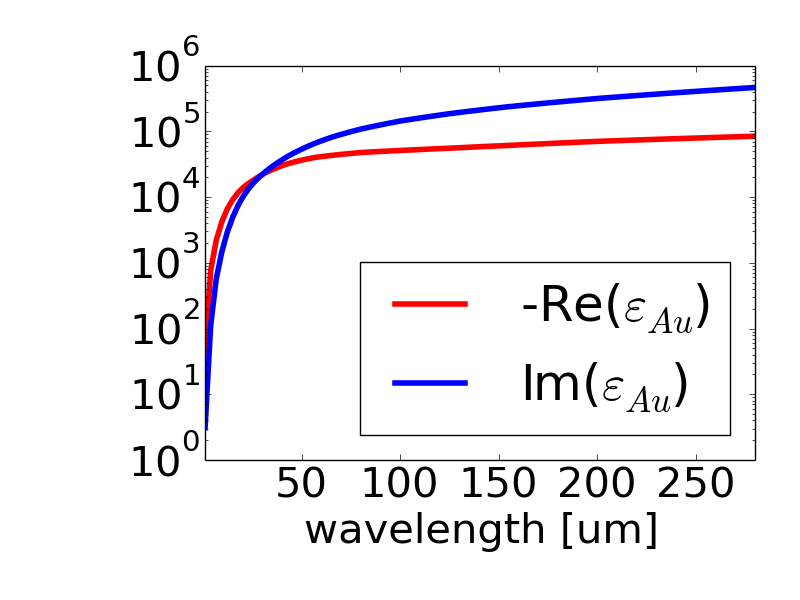
\includegraphics[width=\textwidth]{images/aueps.png}
		\caption{}
		\label{fig:aueps}
	\end{subfigure}
	\begin{subfigure}{.45\textwidth}
		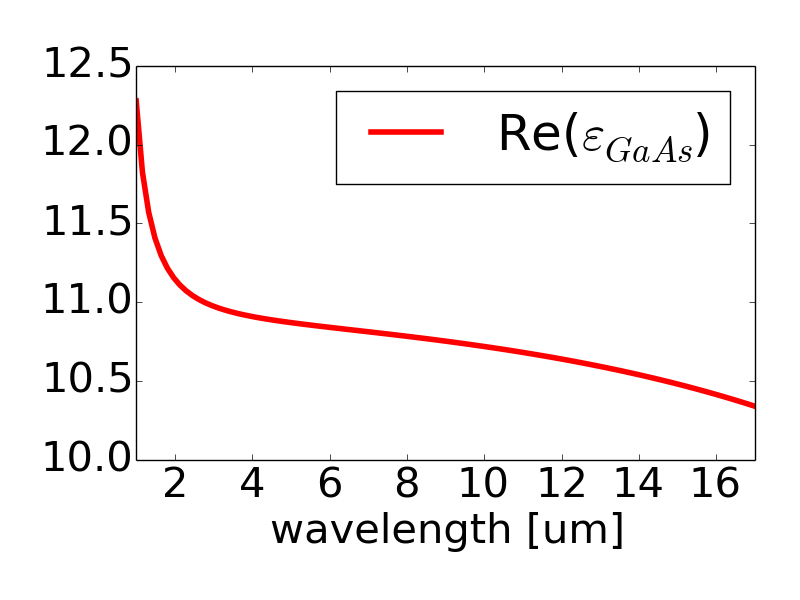
\includegraphics[width=\textwidth]{images/gaaseps.png}
		\caption{}
		\label{fig:gaaseps}
	\end{subfigure}
	\caption{Zależność przenikalności elektrycznej od długości fali dla (a)~$Au$~\cite{ordal1983optical}, (b)~$GaAs$~\cite{skauli2003improved}}
\end{figure}

Różnica wartości bezwzględnej części rzeczywistej i~urojonej przenikalności elektrycznej złota zmniejsza się wraz ze wzrostem częstotliwości. Dla $f=2$~THz moduł części rzeczywistej jest ok. 5 razy mniejszy od modułu części urojonej. Część rzeczywista przenikalności elektrycznej dla fal dłuższych niż optyczne jest ujemna, a jej moduł zmienia się od $10^2$ do $10^4$. Ze względu na dominujący charakter części urojonej związanej z~przewodnictwem, eksperymentalne wyznaczenie przenikalności elektrycznej jest bardzo trudne. Eksperymentalne wyznaczenie części rzeczywistej $\varepsilon_{\textrm{Au}}$ prowadzone jest jedynie dla częstotliwości powyżej $1$~THz~(długości fali poniżej ok. $300$~$\mu$m)~\cite{ordal1983optical}\footnote{Powyższa analiza prawdziwa jest dla eksperymentów prowadzonych w~temperaturze pokojowej. Obniżenie temperatury do~$T=$80K powoduje wzrost przewodności złota do $\sigma_0=208\frac{S}{\mu m}$. W temperaturach kriogenicznych w~cienkich warstwach złota dominujący wpływ na przewodność może mieć rozpraszanie elektronów na defektach struktury~\cite{lide2009crc}}. Zależność $\varepsilon$ od długości fali została przedstawiona na wykresie \ref{fig:aueps}. 

Symulacje opisywane w~poniższym rozdziale prowadzone są z~maksymalną rozdzielczością $0.5$~$\mu$m na punkt obliczeniowy, natomiast głębokość naskórkowa dla $1$~THz, $\delta=74.9$~nm~\cite{lee2009principles}. Mała głębokość naskórkowa w~porównaniu do długości fali oraz rozmiaru siatki przyjętej w~obliczeniach uprawnia do przybliżenia złota przez doskonały przewodnik. 

W przeciwieństwie do złota, warstwy $GaAs$ w~zakresie THz mogą być traktowane jako bezstratne. Charakteryzują się one również słabą dyspersją, a w~przypadku obliczeń prowadzonych dla wąskiego zakresu długości fali, wartość przenikalności elektrycznej może być traktowana jako stała. Warto jednak zwrócić uwagę na to, że warstwy $GaAs$ uzyskiwane w~wyniku epitaksji z~wiązki molekularnej poddawane są zazwyczaj procesowi wygrzewania w~celu ich wygładzenia lub eliminacji zanieczyszczeń. Proces ten może mieć jednak znaczący wpływ na koncentrację elektronów w~paśmie przewodnictwa, co może istotnie zmienić właściwości elektromagnetyczne tego materiału~\cite{zhang2009annealing}. Zależność przenikalności elektrycznej od długości fali dla $GaAs$ przedstawia wykres na rysunku \ref{fig:gaaseps}.

\section{Siatki metalowe pełniące funkcję anteny w~detektorze promieniowania terahercowego}
\subsection{Rezonansowa transmisja przez grube siatki}
\label{subart:rezo-grating}

\begin{figure}[tb]
	\centering
	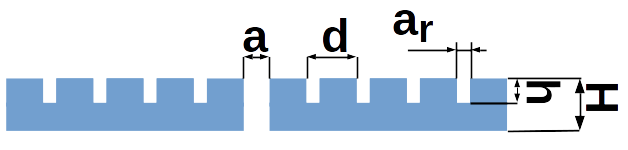
\includegraphics[width=0.9\textwidth]{images/thz/schemat-1szczelina.png}
	\caption{Schemat szczeliny otoczonej siatką rowków w celu umożliwiającej wysoką transmisję rezonansową}
	\label{fig:szczelina-schem}
\end{figure}

\begin{figure}[bt]
	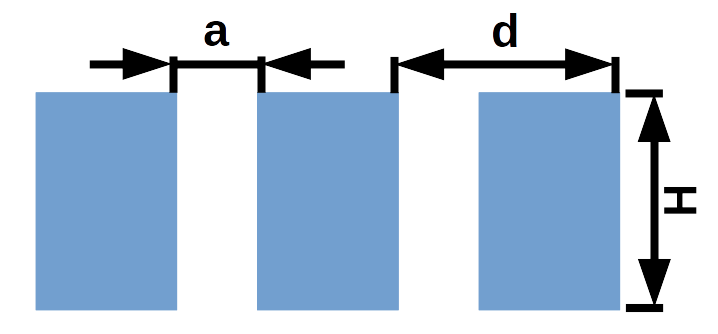
\includegraphics[width=\textwidth]{images/thz/schemat-siatka.png}
	\caption{Schemat siatki dyfrakcyjnej wykorzystywanej w symulacjach}
	\label{fig:rezo-siat-H}
\end{figure}

Modelowym układem, w którym można przeprowadzić analizę zjawisk związanych z rezonansową transmisją fali elektromagnetycznej przez siatkę z idealnego przewodnika jest układ przedstawiony na rysunku \ref{fig:szczelina-schem} oświetlony od strony rowków. Zakładając, że zarówno rowki jak i szczelina są na tyle cienkie, że możliwe jest wzbudzenie w nich jedynie modu podstawowego\footnote{Dla falowodów planarnych metal-izolator-metal nie istnieje długość fali odcięcia dla modu podstawowego w polaryzacji TM}, problem propagacji fali E-M przez układ można rozwiązać analitycznie. W tym celu promieniowanie w przestrzeni swobodnej możemy rozłożyć na fale płaskie, a wzbudzenia wewnątrz rowków i falowodu zastąpić polami modów podstawowych. Wymagając odpowiednich warunków zszycia rozwiązań wzmocnioną transmisję przez szczelinę możemy opisać przy pomocy następujących mechanizmów~\cite{martin2001theory}:
\begin{itemize}
	\item Rezonansowa transmisja przez mod falowodowy w szczelinie. Kontrolowana przez grubość metalu $H$ na zasadzie rezonansu Fabry-P\'{e}rot. Maksimum transmisji występuje w przyjętym przybliżeniu dla
\begin{equation}
\frac{\lambda}{n_{\textrm{eff}}} = 2 \frac {H}{m},
\label{eq:fp-szczelina}
\end{equation}
gdzie $\lambda$ oznacza długość fali promieniowania padającego na układ, $H$ zgodnie z rysunkiem \ref{fig:szczelina-schem} jest długością falowodu, $m$ dowolną liczbą naturalną, a $n_{\textrm{eff}}$ efektywnym współczynnikiem załamania modu falowodowego. W przypadku falowodów metal-powietrze-metal $n_{\textrm{eff}} \approx 1$.
	\item Wzbudzenie modów w rowkach, pozwalające na późniejszy transport energii z rowków do szczeliny przy pomocy fali powierzchniowej. Dzięki temu mechanizmowi transmisja przez szczelinę unormowana do rozmiarów otworu może być znacznie większa od 1. Warunek na rezonansowe wzbudzenie modów wewnątrz szczelin to $\lambda \approx 4 \frac {h}{2m+1}$ (patrz rys. \ref{fig:szczelina-schem}, wykorzystanie tego wzbudzenia możliwe jest jednak jedynie przy dopasowanej reemisji energii z kolejnych rowków.
	\item Zgodne w fazie drgania modów w rowkach, pozwalające na wzbudzenie w płaszczyźnie wejściowej fali powierzchniowej transportującej energię fali E-M do szczeliny. Sytuacja taka występuje dla $d \approx \lambda$.
\end{itemize}



\begin{figure}[tb]
\begin{subfigure}{0.45\textwidth}
	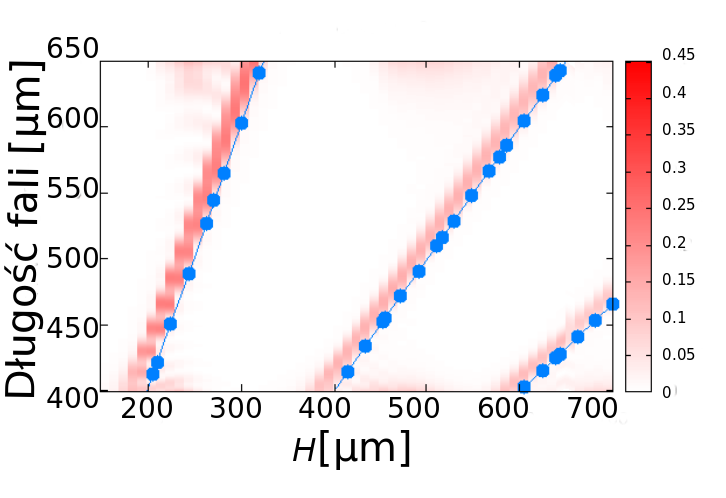
\includegraphics[width=\textwidth]{images/antenaThz/rezonant_trans_f001.png}
	\caption{$f=$99\%,~d=400~$\mu$m }
	\label{fig:rezof001}
\end{subfigure}
\begin{subfigure}{0.45\textwidth}
	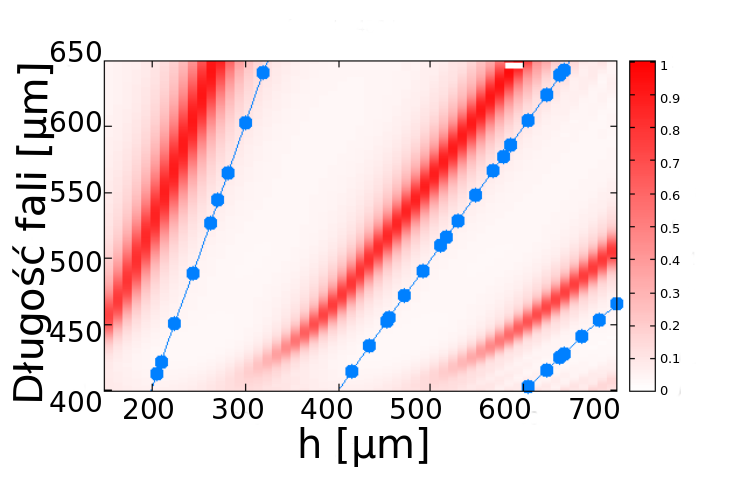
\includegraphics[width=\textwidth]{images/antenaThz/rezonant_trans_f01.png}
	\caption{$f=$90\%,~d=400~$\mu$m }
	\label{fig:rezof01}
\end{subfigure}

\begin{subfigure}{0.45\textwidth}
	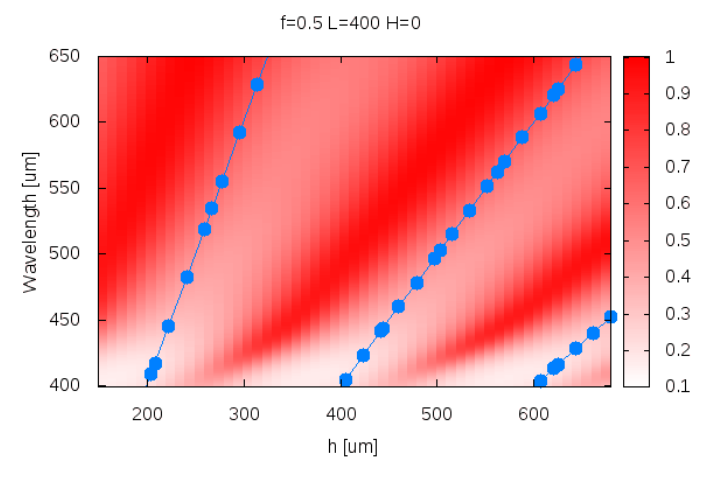
\includegraphics[width=\textwidth]{images/antenaThz/rezonant_trans_f05.png}
	\caption{$f=$50\%,~d=400~$\mu$m }
	\label{fig:rezof05}
\end{subfigure}
\begin{subfigure}{0.45\textwidth}
	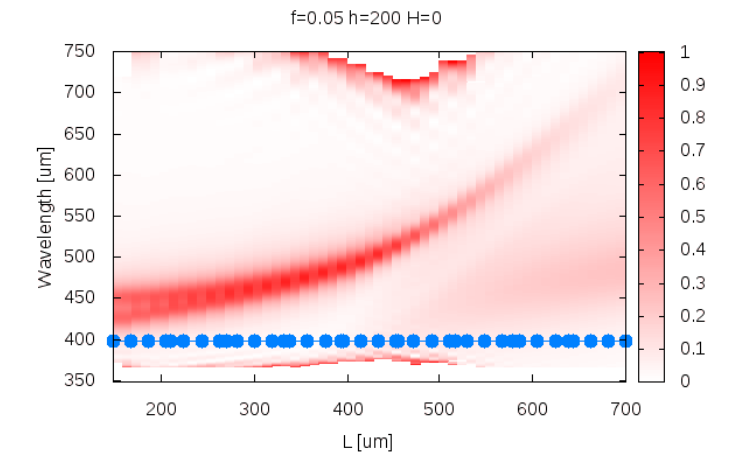
\includegraphics[width=\textwidth]{images/antenaThz/rez_trans_L.png}
	\caption{$f=$90\%,~H=400~$\mu$m}
	\label{fig:rezL}
\end{subfigure}

\caption{Zależność współczynnika transmisji od parametrów geometrycznych siatki. Niebieską linią kropkowaną zaznaczono przewidywane wzorem (\ref{eq:fp-szczelina}) położenie maksimum rezonansu transmisji. }
\label{fig:rezo-siat-H}
\end{figure}

Ze względu na trudności w eksperymentalnej realizacji układu z rysunku \ref{fig:szczelina-schem}, oraz zależności położenia od rezonansu (\ref{eq:fp-szczelina}) jedynie od grubości w kolejnych symulacjach skupiono się na siatce dyfrakcyjnej jak na rysunku \ref{fig:rezo-siat-H}.  Za pomocą symulacji metodą FDTD sprawdzono przewidywane w przybliżeniu cienkich falowodów położenie rezonansu, oraz dokonano ilościowego oszacowania transmisji promieniowania THz przez nieskończoną jednowymiarową metalową siatkę dyfrakcyjną w zależności od jej grubości $H$ i współczynnika wypełnienia $f=\frac{a}{d}$. Wykresy przedstawione na rysunku \ref{fig:rezo-siat-H} wykazują, że nawet dla siatek dyfrakcyjnych o szerokich, chociaż ciągle znacząco podfalowych otworach, jak $a=40$~$\mu$m możliwe jest uzyskanie transmisji rezonansowej. Położenie rezonansu ulega jednak przesunięciu w kierunku większych długości fali \cite{Szczytko2012271}.

Za pomocą symulacji metodą FDTD wykazano również, że wraz ze wzrostem okresu siatki $d$ następuje zarówno przesunięcie maksimum rezonansu w kierunku dłuższych fal, jak i zawężenie transmitowanego pasma. Wydłużenie okresu siatki może więc posłużyć do zawężenia zakresu transmitowanych długości fali przy jednoczesnym powiększeniu otworów. Rozkład energii całkowitej pola E-M uzyskiwanego przy oświetleniu omawianych siatek złotych falą o długości znajdującej się w maksimum transmisji przedstawia rysunek \ref{fig:consrcl525}, natomiast rozkład pola powstający w przypadku źródła odstrojonego od rezonansu przedstawia rysunek \ref{fig:consrcl500}.

\begin{figure}[bth]
	\begin{subfigure}{0.45\textwidth}
		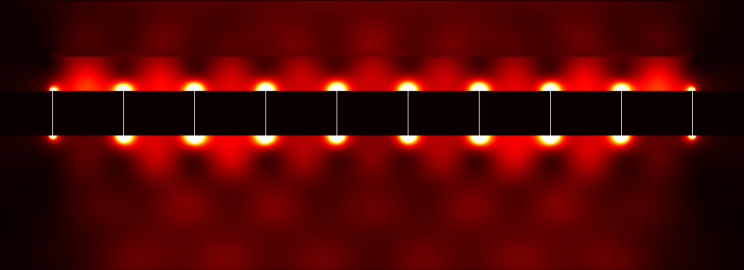
\includegraphics[width=\textwidth]{images/thz/con_src_l525.png}
		\caption{$H=$250~$\mu$m, $\lambda=$525~$\mu$m}
		\label{fig:consrcl525}
	\end{subfigure}
	\begin{subfigure}{0.45\textwidth}
		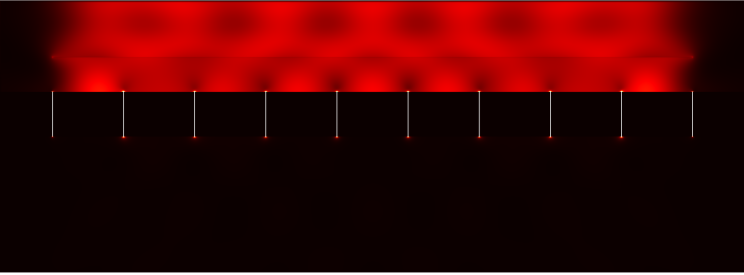
\includegraphics[width=\textwidth]{images/thz/con_src_l500.png}
		\caption{$H=$250~$\mu$m, $\lambda=$500~$\mu$m}
		\label{fig:consrcl500}
	\end{subfigure}
	\caption{Rozkład całkowitej energii pola E-M dookoła siatki złotej oświetlonej z góry za pomocą monochromatycznego źródła o długości fali $\lambda$} 
\end{figure}


\subsection{Antena dla promieniowania THz o~działaniu opartym na wzbudzeniu modu falowodowego}
\label{subart:antenaThz}
Projektowana antena promieniowania THz powinna nie tylko zapewniać selektywność reakcji na promieniowanie E-M z~wąskiego zakresu długości fali, co można uzyskać przy użyciu mechanizmów opisanych w~podrozdziale \ref{subart:rezo-grating}. Jej podstawowym zadaniem jest umożliwiać pobudzenie detektora zlokalizowanego w~małym obszarze za pomocą promieniowania padającego na dowolną część anteny. Zastosowanie siatki dyfrakcyjnej jest wydajną metodą na sprzężenie fali E-M do podkładu. Możliwe jest uzyskanie wydajności sprzężenia promieniowania terahercowego do falowodu krzemowego, dla niektórych częstości przekraczającej 80\%~\cite{roux2002grating}.  Schemat układu anteny, wraz z~podkładem w~którym umieszczony jest detektor promieniowania THz w~postaci tranzystora polowego, przedstawia rysunek \ref{fig:schem-podklad-falo}.
\begin{figure}[tb]
	\centering
	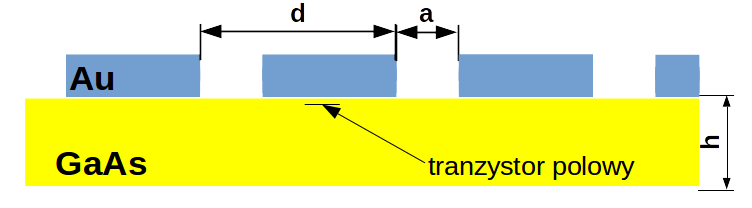
\includegraphics[width=\textwidth]{images/thz/schemat-podklad-falo.png}
	\caption{Schemat detektora promieniowania THz na tranzystorze polowym umieszczonym w~falowodzie z~$GaAs$ z~naniesioną złotą siatką dyfrakcyjną}
	\label{fig:schem-podklad-falo}
\end{figure}

Rozkład pola na rysunku \ref{fig:consrcl525} nie zapewnia transportu promieniowania E-M w~kierunku tranzystora polowego. Możliwy jest jednak transport energii z~wykorzystaniem falowodu planarnego tworzonego przez podkład z~$GaAs$. Ze względu na konieczność stosowania polaryzacji TM w~strukturach opisywanych w~części \ref{subart:rezo-grating}, w~tej części skupiamy się również jedynie na tego typu oświetleniu. Przyjmijmy obecnie, że propagacja fali wzdłuż falowodu odbywa się w~kierunku $z$. Wtedy trzy składowe pola E-M opisujące propagującą się falę to $E_x$,$E_z$ i~$H_y$, które zgodnie z~równaniami Maxwella spełniają układ równań różniczkowych:
\begin{equation}
\begin{gathered}
	\frac{\partial E_x}{\partial z} - \frac{\partial E_z}{\partial x} = -i \mu \omega H_y,\\	
	\frac{\partial H_y}{\partial x} = i~\omega \varepsilon E_z, \\
	- \frac{\partial H_y}{\partial z} = i~\omega \varepsilon E_x.
\end{gathered}
\end{equation}
Z powyższych równań wyprowadzić można równanie różniczkowe drugiego rzędu, będące jedną z~postaci równania Helmholtza, dla składowej $H_y$ w~postaci
\begin{equation}
	\Bigg[ \frac{\partial^2}{\partial x^2} + \frac{\partial^2}{\partial z^2} + \omega^2 \mu_0 \varepsilon_0 \varepsilon (x) \Bigg] H_y = 0,
	\label{eq:waveguide-tm}
\end{equation}
w którym $\varepsilon(x)$ jest kwadratem współczynnika załamania ośrodków. W rozważanym przypadku
\begin{equation}
\varepsilon(x)=  
\begin{cases} 
	1, & \mbox{dla } x>h\mbox{ powyżej podkładu z~GaAs } \\ 
	\varepsilon_{\textrm{GaAs}}, & \mbox{dla } 0<x<h\mbox{ wewnątrz podkładu z~GaAs} \\
	\varepsilon_x,	&	\mbox{dla } x<0\mbox{ poniżej podkładu z~GaAs}.\\
\end{cases}
\end{equation}
W powyższym równaniu współczynnik załamania poniżej struktury został opisany jako $\varepsilon_x$, co pozwala w~dalszej analizie rozważać falowody, w~których $GaAs$ zostało umieszczone na innym materiale. Szukając rozwiązań równania (\ref{eq:waveguide-tm}) w~postaci fal płaskich, propagujących się wewnątrz rdzenia ($0<x<h$) wzdłuż osi z:
\begin{equation}
	H_y(x,z)=H_y(x) \textrm{exp}(-i \beta z),
\end{equation}
oraz w~postaci fal zanikających na zewnątrz rdzenia, otrzymujemy równanie zwyczajne
\begin{equation}
	\frac{d H_y^2(x)}{dx^2} + [ k_0^2 \varepsilon - \beta^2 ] H_y = 0.
\end{equation}
Natępnie, stosując standardowe warunki zszycia otrzymujemy równanie dyspersyjne modów prowadzonych w~postaci~\cite{petykiewicz1989podstawy}:
\begin{equation}
tg( \kappa h)=\frac{\kappa [ \delta (\frac{n_{\textrm{GaAs}}}{n_x})^2 + \gamma n_{\textrm{GaAs}}^2 ]}{\kappa^2 - \gamma \delta (\frac{n_{\textrm{GaAs}}}{n_x })^2},
\label{eq:tm-disp}
\end{equation}
gdzie przez $n_{\textrm{GaAs}}$ i~$n_x$ oznaczono odpowiednio współczynnik załamania warstwy arsenku galu, oraz podkładu. Wprowadzono również dodatkowe oznaczenia w~postaci
\begin{equation}
	\begin{gathered}
		\delta=\sqrt{\beta^2-\omega^2 \mu_0 \varepsilon_0 \varepsilon_x},\\
		\gamma=\sqrt{\beta^2-\omega^2 \mu_0 \varepsilon_0},\\
		\kappa=\sqrt{\omega^2 \mu_0 \varepsilon_0 \varepsilon_{\textrm{GaAs}} - \beta^2}.
	\end{gathered}
\end{equation}

Wszystkie wartości $\beta$ spełniające  równanie (\ref{eq:tm-disp}) są dopuszczalnymi wartościami składowej wektora falowego w~kierunku propagacji. W ten sposób efektywne współczynniki załamania modów TM w~falowodzie planarnym można obliczyć jako $n_{\textrm{eff}}=\frac{\beta}{k_0}$. Rozwiązanie powyższego równania możliwe jest jedynie na drodze numerycznej~(rozwiązanie przybliżone można też skonstruować graficznie). W przypadku rozważanych podkładów z~$GaAs$,o gróbości $h=400$~$\textrm{\mu} m$, możliwe wartości efektywnego współczynnika załamania przedstawia wykres \ref{fig:gaas-effn}. Różne współczynniki $n_{\textrm{eff}}$ odpowiadające tej samej długości fali wynikają z~wielomodowego charakteru falowodu tworzonego przez podkład $GaAs$. Dopasowanie pędowe między modem prowadzonym w~falowodzie, a falą padającą wymaga dodania odpowiedniego pędu do fali padającej przez siatkę dyfrakcyjną, co dla składowych wektora falowego możemy zapisać jako
\begin{equation}
k_{i \parallel} + l \frac{2\pi}{d} = k_0 \cdot n_{\textrm{eff,m}} , 
\end{equation}
gdzie przez $k_{i \parallel}$ oznaczono składową wektora falowego fali padającej równoległą do kierunku propagacji w~falowodzie, $l$ jest liczbą całkowitą odpowiadającą rzędowi ugięcia na siatce dyfrakcyjnej, a $n_{\textrm{eff,m}}$ jest efektywnym współczynnikiem załamania m-tego modu falowodowego. W przypadku padania normalnego pęd fali padającej w~kierunku propagacji w~falowodzie wynosi zero. Szczególnie interesujący jest również przypadek wzbudzenia modu za pomocą pierwszego rzędu dyfrakcyjnego siatki, ponieważ dla niego uzyskamy największą wydajność, dlatego po uproszczeniu z~powyższego równania możemy wyprowadzić
\begin{equation}
d=\frac{2 \pi}{k_0 \cdot n_{\textrm{eff,m}}}.
\label{eq:d-do-wzbudzenia}
\end{equation}
Na podstawie powyższego wzoru przygotowano wykres zależności okresu siatki $d$ potrzebnej do wzbudzenia kolejnych modów falowodowych, w~zależności od długości fali, dla której pracować ma antena. Wyniki tych obliczeń przedstawia wykres \ref{fig:d-lusok}.

\begin{figure}
\begin{subfigure}{0.5\textwidth}
        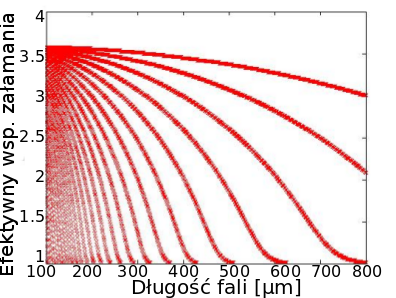
\includegraphics[width=\textwidth]{images/thz/gaas-neffeps.png}
	\caption{}
	\label{fig:gaas-effn}
\end{subfigure}
\begin{subfigure}{0.5\textwidth}
        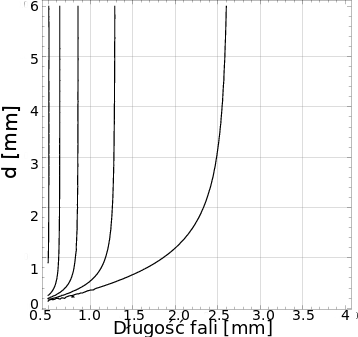
\includegraphics[width=\textwidth]{images/antenaThz/d_lambda.png}
	\caption{}
	\label{fig:d-lusok}
\end{subfigure}
\caption{Wyniki rozwiązania problemu sprzęgania fali do falowodu planarnego o~grubości $h=$400~$\mu$m z~GaAs za pomocą siatki dyfrakcyjnej.  (a) Zależność efektywnego współczynnika załamania $n_{\textrm{eff}}$ od długości fali, (b)~wykres łączący okres siatki dyfrakcyjnej z~długością fali, dla której pracuje antena. }
\end{figure}

\begin{figure}[tb]
	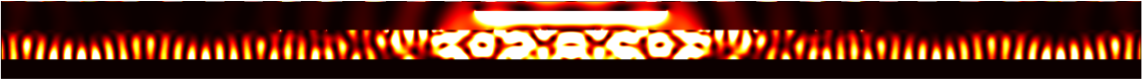
\includegraphics[width=\textwidth]{images/thz/consrc_siatka1d_300GHz_d729um.png}
	\caption{Uzyskany za pomocą symulacji metodą FDTD, uśredniony rozkład gęstości energii pola elektromagnetycznego wewnątrz falowodu z~$GaAs$ o grubości~h=400$~\mu$m, na którym umieszczono antenę w~postaci siatki dyfrakcyjnej o okresie~$d=$729~$\mu$m oświetloną pod kątem normalnym za pomocą źródła o~częstotliwości 300~GHz.  }
	\label{fig:consrc_1d_f300Ghz}
\end{figure}

\begin{figure}[tb]
	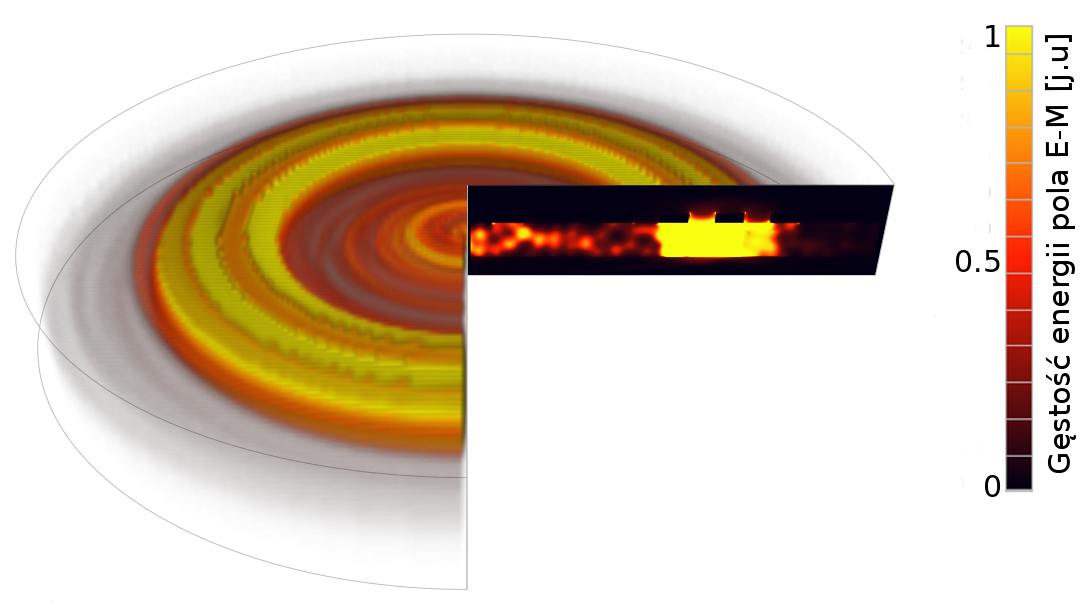
\includegraphics[width=\textwidth]{images/antenaThz/tort.png}
	\caption{Rozkład energii pola E-M uzyskany w~symulacji metodą BOR FDTD wewnątrz falowodu planarnego z~siatką o~geometrii cylindrycznej umieszczoną na podkładzie z~$GaAs$. Wynik symulacji znajduje się w~przekroju przedstawionym na rysunku. Obrazowe przejście do geometrii cylindrycznej uzyskano przez wizualizację średniej wartości w~danym punkcie falowodu.}	
	\label{fig:concent_modfalo}
\end{figure}

Na podstawie przeprowadzonych obliczeń zaprojektowano siatkę ze złota dla źródła o~częstotliwości $f=300$~GHz ($\lambda\approx 1$~mm) o~grubości $H=1$~$\mu$m i~okresie $d=729$~$\mu$m. W strukturach wytwarzanych eksperymentalnie pod podkładem $GaAs$ znajduje się warstwa $Au$ o~grubości 1~$\mu$m, którą w~symulacji metodą FDTD traktujemy jako doskonały przewodnik. Na rysunku \ref{fig:consrc_1d_f300Ghz} przedstawiono rozkład gęstości energii wewnątrz zaproponowanej struktury. Wyniki symulacji komputerowych potwierdzają  możliwość propagacji promieniowania E-M z~zakresu subterahercowego w~kierunku detektora w~zaprojektowanym układzie.
Bazując na pracach numerycznych dotyczących  jednowymiarowych siatek dyfrakcyjnych pozwalających na wzbudzenie modów falowodowych w~podkładach z~$GaAs$, przeanalizowane zostało działanie analogicznych falowodów opartych na cylindrycznych siatkach dyfrakcyjnych. Ze względu na wzbudzenie modów falowodowych o~kierunku propagacji prostopadłym do pasków siatki dyfrakcyjnej uzyskujemy częściową koncentrację promieniowania w~obszarze detektora. Odpowiedni eksperyment numeryczny został przeprowadzony przy użyciu metody BOR-FDTD we współrzędnych cylindrycznych, szerzej opisanej w~podrozdziale \ref{subart:borfdtd}. Wyniki symulacji przedstawione na rysunku \ref{fig:concent_modfalo} odpowiadają strukturze z~$GaAs$ o~rozmiarach 10x10mm pokrytej siatką dyfrakcyjną o~okresie $d=538$~$\mu$m i~otworach o~szerokości $250$~$\mu$m (współczynnik wypełnienia $f=0.53$), która została oświetlona promieniowaniem o~długości fali $\lambda=2.52$~mm. W ten sposób potwierdzono możliwość wykorzystania tego typu struktur do konstrukcji anten dla detektorów promieniowania THz umieszczonych wewnątrz podkładu z~$GaAs$~\cite{Stolarek2011}.


\section{Transmisja jednokierunkowa}
Najszerzej znanymi elementami fotonicznymi, które charakteryzują się jednokierunkową transmisją światła są izolatory Faradaya.  Podstawą ich działania jest zjawisko Faradaya, polegające na obrocie płaszczyzny polaryzacji światła przechodzącego przez ośrodek magnetooptyczny w~obecności zewnętrznego pola magnetycznego. W~tej pracy będziemy się zajmować możliwością uzyskania asymetrycznej transmisji w strukturach złożonych z~metalowych siatek, w~których nie występuje zjawisko magneto-optyczne, ani zjawiska nieniowe. Na podstawie tw.~o~wzajemności Lorentza można wykazać, że takie układy nie mogą być izolatorami rozumianymi w~takim sensie, że jeśli opiszemy je używając macierzy rozpraszania do opisu zależności między wejściami i wyjściami układu, zawsze otrzymamy macierz symetryczną~\cite{4171512}. Jednocześnie okazuje się, że twierdzenie to nie stoi to w sprzeczności z możliwością blokowania transmisji światła dla padania z jednej strony siatki i przepuszczania światła przy przeciwnym kierunku padania~\cite{lockyear2006one}.

W dalszej części tego rozdziału omawiane są podwójne metalowe siatki dyfrakcyjne~(ang. DMG - double metallic grating)\nomenclature{DMG}{ang. Double Metallic Grating - podwójna metalowa siatka dyfrakcyjna}. Dla rozróżnienia, w~odniesieniu do wcześniej omawianych siatek wykorzystywany jest termin SMG~(ang. single metallic grating).

\begin{figure}[tb]
	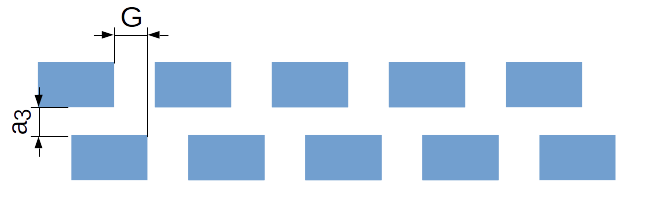
\includegraphics[width=\textwidth]{images/dmg/dmg_general_schem.png}
	\caption{Schematyczny obraz siatki DMG analizowanej w~pracy~\cite{cheng2007controllable}}
	\label{fig:cheng_dmg_schem}
\end{figure}

Przykład struktury typu DMG zbudowanej z~dwu siatek dyfrakcyjnych o~tym samym współczynniku wypełnienia i~okresie przedstawia rysunek~\ref{fig:cheng_dmg_schem}. Propozycję tego typu struktury jako uogólnienia SMG podał Chen Cheng i~inni~\cite{cheng2007controllable}, prezentując możliwość regulacji położenia maksimum widma transmisji przez dobór względnego usytuowania siatek. Zgodnie ze schematem na rysunku \ref{fig:cheng_dmg_schem} rozsunięcie siatek opisywane jest dwoma parametrami $G$ i~$a_3$. Możliwe jest uzyskanie niskiej transmisji przez strukturę dla szerokiego zakresu widmowego przy odpowiednim doborze względnego położenia siatek, co może zostać wykorzystane do budowy urządzeń mikromechanicznych kontrolujących współczynnik transmisji wiązki~\cite{cheng2007controllable}.

Analizę fizycznych mechanizmów prowadzących do nadzwyczajnej transmisji przez DMG zaczniemy od przypadku $a_3=0$ i~$G=0$. W takiej sytuacji uzyskujemy strukturę SMG o~grubości dwóch siatek składających się na DMG. Zgodnie z~wykresami na rysunku~\ref{fig:rezo-siat-H} dla tego typu siatki złożonej z~dwóch SMG o~grubości $h=300$~$\mu$m (por. rys. \ref{fig:schem-podklad-falo}) uzyskalibyśmy rezonanse transmisji takie jak dla siatki o~$h=600$~$\mu$m, czyli dla długości fali $\lambda \approx 400$~$\mu$m~i~$\lambda \approx 600$~$\mu$m. W wyniku stopniowego zwiększania odległości $a_3$ obserwujemy zbliżanie obu maksimów transmisji~\cite{cheng2008physical}. W odległość $a_3 \approx \frac{h}{2}$, następuje degeneracja obu modów, a maksimum transmisji występuje w~okolicach maksimów transmisji obu siatek SMG dla $\lambda \approx 560$~$\mu$m \cite{cheng2008physical}. Dalsze zwiększanie odległości powoduje znaczący spadek transmisji w~szerokim zakresie widma długości fali. Związane jest to ze słabym sprzężeniem stojącej fali powierzchniowej za pierwszą siatką SMG z~modami falowodów w~drugiej siatce SMG. Znaczne zwiększenie $a_3$, aż do odległości odpowiadającej warunkowi konstruktywnej interferencji w~rezonatorze Fabry-Perot tworzonego przez powietrze i~dwie warstwy o~efektywnych współczynnikach i~grubościach obliczonych zgodnie z~modelem efektywnym przedstawionym w~pracy \cite{shen2005mechanism} prowadzi do powstania kolejnych maksimów transmisji przez cały układ.

Niezależnie od modyfikowania własności transmisyjnych za pomocą odległości $a_3$ między siatkami SMG, przesunięcie maksimum transmisji jak i~jej blokowanie, można uzyskać zmieniając boczne przesunięcie siatek - $G$. Maksimum transmisji przez DMG można uzyskać również dla układu, w~którym $G$ dobrano tak, aby wyeliminować bezpośredni prześwit przez strukturę. Dla DMG jak na rysunku~\ref{fig:cheng_dmg_schem}, maksimum transmisji przez strukturę występuje dla $G$ równego zero lub połowie okresu SMG. Minimum transmisji napotykamy natomiast dla $G$ równego ćwierć okresu SMG~\cite{chan2006optical}.

\begin{figure}[tb]
	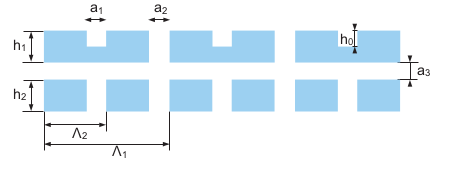
\includegraphics[width=\textwidth]{images/thz/1D-DMG-schemat.png}
	\caption{Schemat podwójnej siatki metalowej DMG zaprojektowanej do uzyskania transmisji asymetrycznej}
	\label{fig:1ddmg-schem}
\end{figure}


Możliwość zastosowania podwójnych siatek metalowych w~celu uzyskania różnej transmisji w~przypadku propagacji światła w~przeciwnych kierunkach przez strukturę zostało zaproponowane przez Ji Xu i~innych \cite{xu2011unidirectional}. W przeciwieństwie do wcześniejszych prac na temat DMG~\cite{cheng2007controllable,cheng2008physical,chan2006optical} w~zaproponowanej strukturze jedna z~siatek miała okres większy od długości fali dla której projektowano układ ($\Lambda>\lambda$). Autorzy błędnie interpretując wyniki symulacji FDTD twierdzili, że możliwe jest zastosowanie tego typu struktury jako elementu toru optycznego o~jednokierunkowej transmisji światła. Późniejsza wykonana przez nas analiza numeryczna i~eksperymentalna wykazała, że układ spełnia twierdzenie Lorenza o~wzajemności - w~związku z~czym nie może być  traktowany jako izolator optyczny \cite{jalas2013and}. Zwiększenie okresu jednej z~siatek umożliwiło zastosowanie rowków w~siatce wejściowej dla kierunku charakteryzującego się wysokim współczynnikiem transmisji~\cite{xu2011unidirectional}.

Odpowiednio dobrane parametry siatki podwójnej mogą prowadzić jednak do transmisji asymetrycznej. Różnica w~transmisji przejawia się niskim współczynnikiem transmisji przy oświetleniu prostopadłym jednej ze stron i~wysokim przy oświetleniu z~drugiej. Nie jest to jednak warunek wystarczający na realizację izolatora optycznego \cite{jalas2013and}, ponieważ w~przypadku wysokiej transmisji promieniowanie E-M jest uginane przez siatkę dyfrakcyjną. 

\begin{figure}[tb]
	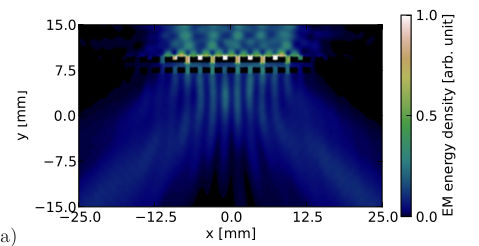
\includegraphics[width=\textwidth]{images/thz/opt_lett_gora.png}
	\caption{Rozkład gęstości energii pola E-M w~przypadku prostopadłego oświetlenia układu DMG zaprojektowanego do transmisji asymetrycznej od strony siatki z~rowkami~\cite{Stolarek:13}}
	\label{fig:trans_gora}
\end{figure}

\begin{figure}[tb]
	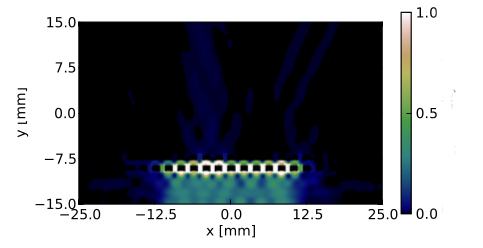
\includegraphics[width=\textwidth]{images/thz/opt_letters_dol.png}
	\caption{Rozkład gęstości energii pola E-M w~przypadku prostopadłego oświetlenia układu DMG zaprojektowanego do transmisji asymetrycznej od strony siatki podfalowej~\cite{Stolarek:13} }
	\label{fig:trans_dol}
\end{figure}

Fakt ten wynika z~budowy podwójnej siatki metalowej służącej do uzyskania transmisji asymetrycznej, która została przedstawiona na rysunku \ref{fig:1ddmg-schem}. Uzyskanie transmisji jednokierunkowej możliwe jest przy dobraniu parametrów układu tak, aby $\Lambda_1 = 2\Lambda_2$ oraz długość fali E-M $\lambda$ padającej na DMG  spełniała nierówność $\Lambda_2<\lambda<\Lambda_1$. Przywołując klasyczne prawo Braggów
\begin{equation}
	\Lambda \cdot \textrm{sin}(\alpha_k) = k \lambda,
\end{equation}
gdzie $\Lambda$ oznacza okres siatki dyfrakcyjnej, $k$ jest liczbą całkowitą numerującą rząd dyfrakcyjny padający pod kątem $\alpha_k$, a $\lambda$ długością padającej płaskiej fali E-M. Dla padania pod kątem $0^{\circ}$, zakładając otoczenie w~postaci powietrza z~obu stron DMG możemy wyprowadzić warunek na liczbę rzędów ugięcia uzyskiwanych przy użyciu siatki dyfrakcyjnej o~okresie $\Lambda$. 
\begin{equation}
	 0 \le |k| \le \frac { \Lambda }{\lambda},
\end{equation}
z którego wynika, że omawiany układ może wykazywać jednie -1,~0~i~+1 rząd ugięcia dla  $\Lambda=\Lambda_1$. Ze względu na podfalowy okres $\Lambda_2$ fala E-M padająca pod kątem $0^{\circ}$ będzie przez tę siatkę propagować się bez zmiany kierunku.  W wyniku interferencji za siatką dyfrakcyjną o~okresie $\Lambda_1$ możliwe jest wyeliminowanie jednego z~rzędów dyfrakcyjnych. Przedstawiona siatka projektowana jest dla długości fali $\lambda \approx 2.9$~mm, dla której kąt ugięcia $-1$~i~$+1$ rzędu wynosi $\alpha_{\pm 1} = 45^{\circ}$, która charakteryzuje się wygaszeniem rzędu zerowego. Wynik symulacji FDTD przedstawiający rozkład energii pola E-M w~przypadku oświetlenia struktury od strony siatki o~okresie $\Lambda_1$ przedstawia rysunek \ref{fig:trans_gora}.

\begin{SCfigure}
	\centering
	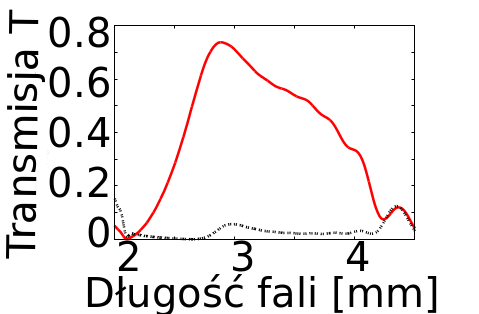
\includegraphics[width=0.5\textwidth]{images/thz/opt_lett_spect.png}
	\caption{Zależność współczynnika transmisji przez omawianą strukturę DMG od długości fali dla oświetlenia z~różnych stron. Wykres odpowiada DMG o~$\Lambda_1= 2 \Lambda_2 = 4.2$~mm, $a_1=a_2=a_3=0.7$~mm, $h_1=h_2=2 h_0=1$~mm~\cite{Stolarek:13}.}
	\label{fig:trans_freq}
\end{SCfigure}

 W innym ujęciu, strukturę typu DMG można analizować jako układ falowodów metal-dielektryk-metal, o~rozmiarach podfalowych ( $a_1,a_2,a_3 < \lambda$), dlatego wzbudzany może być w~nich jedynie mod podstawowy w~polaryzacji TM. Promieniowanie o~polaryzacji TE jest w~pełni odbijane przez omawiany układ. Dla $h_1=h_0$ i $a_3 \to 0$ struktura przypomina siatkę omawianą w~podrozdziale \ref{subart:rezo-grating} przedstawioną na rysunku \ref{fig:rezo-siat-H}. W przypadku $a_3 \ne 0$ możliwe jest dodatkowe sprzęganie pomiędzy falowodami poprzez falowód powstający pomiędzy siatkami dyfrakcyjnymi. Różnica w~fazie składowych pola E-M dochodzącego do otworów w~siatce o~okresie $\Lambda_1$ w~przypadku oświetlenia prostopadłego od strony siatki o~okresie $\Lambda_2$ w~omawianym przypadku wynosi $\pi$, w~wyniku czego współczynnik transmisji dla takiej sytuacji zbliża się do~0. Rozkład gęstości energii odpowiadający oświetleniu układu od strony siatki o~okresie $\Lambda_2$ przedstawia rysunek \ref{fig:trans_dol}.

W wyniku optymalizacji numerycznej parametrów struktury, prowadzonej za pomocą serii symulacji metodą FDTD, w~których parametry struktury podlegały ewolucji na bazie algorytmu genetycznego, uzyskano dla szerokiego zakresu długości fali znaczącą różnicę współczynników transmisji dla oświetlenia z~różnych stron DMG~\cite{Stolarek:13}. Zależność współczynnika transmisji przez DMG w~przeciwnych kierunkach od długości fali przedstawia wykres na rysunku \ref{fig:trans_freq}. Dalsze symulacje numeryczne wykazały, że możliwa jest niezależna zmiana otworów w~obu siatkach bez utraty transmisji jednokierunkowej w~celu poprawy kontrastu standardowo wyrażanego wzorem
\begin{equation}
C=\frac{|T_1 - T_2|}{T_1+T_2},
\label{eq:contrast}
\end{equation}
gdzie przez $T_1$ i~$T_2$ oznaczono natężeniowe współczynniki transmisji przy oświetleniu DMG odpowiednio od strony siatki o~okresie $\Lambda_1$ i~$\Lambda_2$.

Dla pełnego zrozumienia znaczenia kontrastu wprowadźmy dodatkowe definicje:
\begin{equation}
	\begin{gathered}
	R=T_1-T_2, \\
	Q=\frac{T_1}{T_2}.
	\end{gathered}
	\label{eq:rq-def}
\end{equation}
Zakładając, że $T_1>T_2$ (z czego wynika, że $Q>1$), możemy zapisać wyrażenie z~mianownika wzoru (\ref{eq:contrast}) za pomocą wprowadzonych zmiennych $R$ i~$Q$:
\begin{equation}
	T_1+T_2=\frac{Q+1}{Q-1} \cdot R,
\end{equation}
co po podstawieniu do wzoru (\ref{eq:contrast}) wskazuje, że pomimo tego, że różnica transmisji $R$  znajduje się w~liczniku wyrażenia, to sam kontrast zależny jest jedynie od ilorazu transmisji w~przeciwnych kierunkach i~wyraża się wzorem:
\begin{equation}
	C=\frac{Q-1}{Q+1}
	\label{eq:contrast-Q}.
\end{equation}
Oznacza to, że oprócz kontrastu $C$, przy analizie transmisji należy posługiwać się także transmisją $T_1$ lub różnicą $R$~\cite{stolarek2013broadband}. Równoważnie można prowadzić optymalizację tego typu struktury wykorzystując do tego wprowadzone oznaczenia $R$ i~$Q$. Dla odróżnienia od poprzednich siatek, w~których otwory w~obu siatkach SMG były równe $a_2$, wprowadzono oznaczenia $d_1$ i~$d_2$ - dla otworów w~siatkach o~okresie odpowiednio $\Lambda_1$ i~$\Lambda_2$. Zależność wprowadzonych w~(\ref{eq:rq-def}) współczynników od długości fali i~rozmiarów otworów przedstawiają wykresy na rysunku \ref{fig:qr-od-d}.

\begin{figure}[tb]
	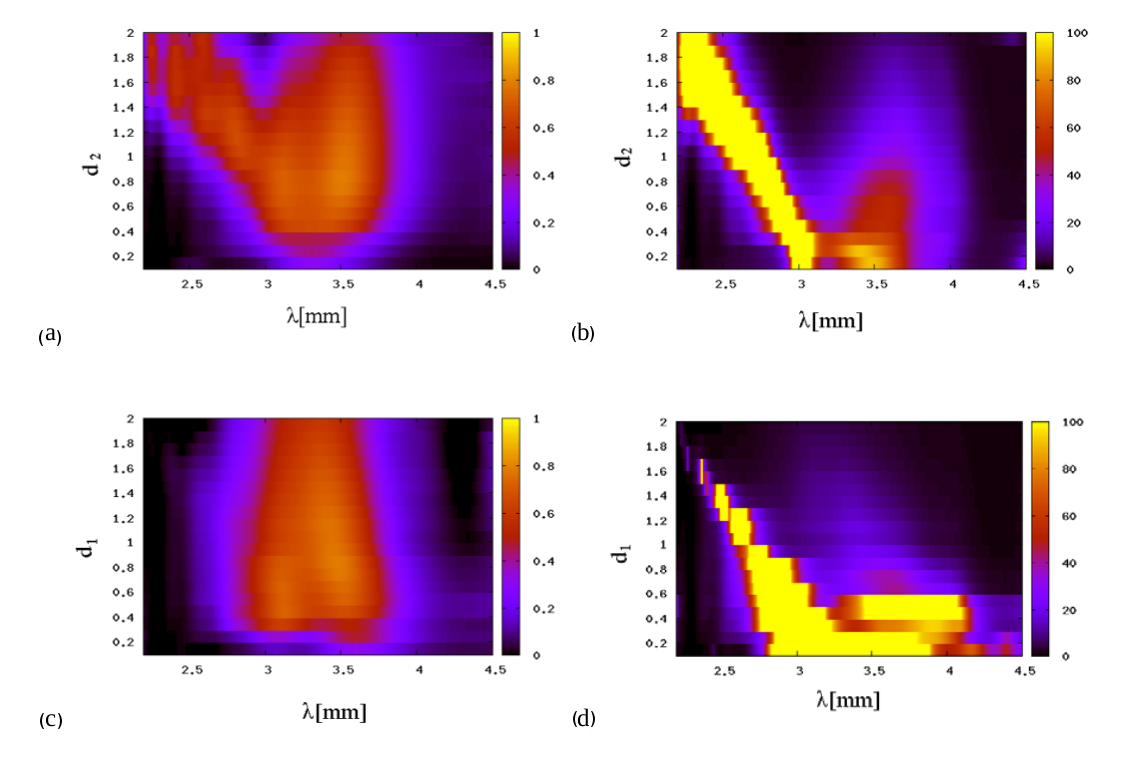
\includegraphics[width=\textwidth]{images/dmg/kontrast_maps.png}
	\caption{Zależność współczynników $R$ (a) i~(c), oraz $Q$ (b) i~(d) od długości fali $\lambda$ oraz od rozmiarów otworów w~obu siatkach. Rozmiar otworów dla (a) i~(b) jest   jest równy $d_1=0.7$~mm, natomiast dla (c) i~(d) $d_2=0.7$~mm }
	\label{fig:qr-od-d}
\end{figure}

Oczekiwane parametry pracy wielowarstwy to $R=1$ oraz $Q \to \infty$ oznaczające transmisję jednokierunkową. Na podstawie wyników zaprezentowanych na rysunku \ref{fig:qr-od-d} możemy stwierdzić, że optymalnymi rozmiarami otworów są $d_1\in(0.3,0.5)$~mm, oraz $d_2\in(0.6,1)$~mm w~przypadku pracy układu dla długości fali z~zakresu $\lambda \in (2.5, 4)$mm. Dodatkowo stwierdzić można, że
\begin{itemize}
	\item Zwiększanie $d_1$ powyżej wskazanego zakresu powoduje znaczne zwiększenie transmisji w~kierunku blokującym - co objawia się spadkiem kontrastu na wykresie \ref{fig:qr-od-d}d.
	\item Zmiana rozmiaru $d_2$ nie ma zasadniczego wpływu na $Q$, a tym samym na kontrast (\ref{eq:contrast-Q}), może jednak prowadzić do poszerzenia widma i~zwiększenia różnicy $R$ transmisji w~przeciwnych kierunkach (patrz rysunek \ref{fig:qr-od-d}a).
	\item Dla wąskiego zakresu długości fali w~okolicach $\lambda\approx2.6$~mm, możliwe jest uzyskanie wysokiego kontrastu $Q>100$ i~różnicy ${R\approx 0.7}$, dla ${d_1>1}$~mm. Taka struktura wykazuje jednak transmisję wynoszącą ok.~10\% dla fal dłuższych od $3$~mm~\cite{stolarek2013broadband}.
\end{itemize}

\section{Soczewka dyfrakcyjna o~transmisji jednokierunkowej}
\begin{figure}
	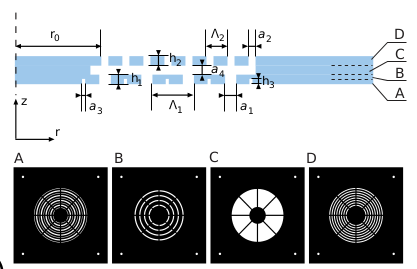
\includegraphics[width=\textwidth]{images/dmg/express_siatki.png}
	\caption{Schemat DMG w~konfiguracji cylindrycznej uzyskiwanej przez złożenie wielu przesłon o~grubości $\frac{\lambda}{30}$ \cite{Yavorskiy:14}}
	\label{fig:schem-cyl}
\end{figure}

Transmisja w~-1~i~+1 rzędzie dyfrakcyjnym przez strukturę jednowymiarową opisywaną w~poprzedniej części pracy może zostać wykorzystana do koncentracji wiązki. 

W omawianej wcześniej geometrii planarnej za siatką obserwowaliśmy obszary konstruktywnej i~destruktywnej interferencji z~kolejnych otworów siatki. W niniejszym podrozdziale analizowana jest podwójna siatka dyfrakcyjna, która umożliwia koncentrację promieniowania za pomocą mechanizmu przypominającego działanie płytki strefowej Fresnela. Analogię między geometrią planarną, a cylindryczną możemy odnaleźć poprzez myślowe przedstawienie siatki jednowymiarowej jako fragmentu siatki o~bardzo dużym promieniu $r$. Ze względu na konieczność oświetlenia DMG za pomocą promieniowania E-M, którego natężenie pola magnetycznego $H$ jest w~każdym punkcie równoległe do szczelin siatki, niezbędne w~geometrii cylindrycznej jest wykorzystanie źródła fali E-M o~polaryzacji radialnej. 


W celu eksperymentalnej realizacji jednokierunkowej soczewki dyfrakcyjnej dla promieniowania THz, zaprojektowane zostały przesłony o~grubości $\frac{\lambda}{30}=0.1$~mm, układane w~stos jak na rysunku \ref{fig:schem-cyl}. Zostały one wykorzystane do budowy cylindrycznej wersji struktury typu DMG~\cite{Yavorskiy:14}. 
\begin{figure}[tb]
	\begin{subfigure}{\textwidth}
		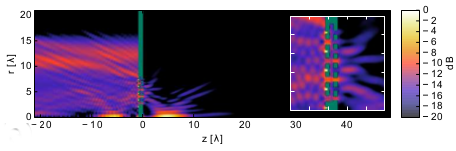
\includegraphics[width=\textwidth]{images/dmg/express-high-kontrast-trans.png}
		\caption{}
	\end{subfigure}

	\begin{subfigure}{\textwidth}
		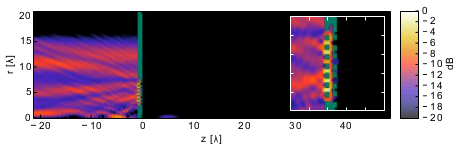
\includegraphics[width=\textwidth]{images/dmg/express-high-kontrast-block.png}
		\caption{}
	\end{subfigure}
	\caption{Rozkład gęstości energii pola E-M dla cylindrycznej siatki DMG oświetlonej falą o~płaskim froncie falowym od strony wykazującej (a) wysoką transmisję i~koncentrację oraz (b) brak transmisji fali padającej~\cite{Yavorskiy:14}. Wewnątrz wykresów przedstawione zostały powiększone obrazy rozkładu gęstości energii w~pobliżu struktury.}
	\label{fig:cyl-gest-ene}
\end{figure}

Układ poddany później weryfikacji doświadczalnej i~obliczeniowej składał się z~dwóch siatek dyfrakcyjnych zawierających odpowiednio 4 i~8 otworów. Okresy siatek wynosiły $\Lambda_1=\frac{4}{3} \lambda$ i~$\Lambda_2=\frac{2}{3} \lambda$, rozmiary otworów to odpowiednio $a_1=\frac{1}{3}\lambda$ i~$a_2=0.267 \lambda$. Odległość od osi symetrii układu do pierwszej szczeliny wynosiła $r_0=2.67\lambda$. Grubości obu siatek były sobie równe $h_1=h_2=\frac{1}{3}\lambda$, a odległość między nimi $a_4=0.233\lambda$. Dodatkowe rowki wzmacniające transmisję miały szerokość $a_3=0.133\lambda$ i~głębokość $h_3=\frac{h_1}{2}$. 

Taka struktura oświetlona została falą o~polaryzacji radialnej o~profilu amplitudy opisanym za pomocą funkcji supergaussowskiej $A \propto \textrm{exp}\{\frac{-(r-R_0)}{2\sigma^2}\}^{10}$, będącej numerycznym odpowiednikiem fali płaskiej we współrzędnych cylindrycznych\footnote{Rozumiemy przez to, że wiązka supergaussowska we współrzędnej radialnej $r$~zawiera znacznej szerokości płaski front falowy o~jednorodnym natężeniu.}. Rozkład gęstości energii odpowiadający opisanej symulacji przedstawia rysunek \ref{fig:cyl-gest-ene}. Na podstawie symulacji FDTD z~impulsem gaussowskim wyznaczono współczynnik kontrastu struktury (\ref{eq:contrast}) równy $C=99.8\%$~\cite{Yavorskiy:14}. Ponieważ metal tworzący podwójną siatkę metalową opisywany jest w~symulacji jako doskonały przewodnik, wykonane obliczenia są, w~granicach stosowalności tego przybliżenia, skalowalne z~długością fali.

\begin{figure}
	\centering
	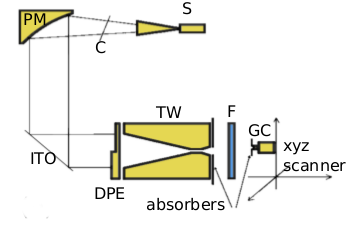
\includegraphics[width=0.5\textwidth]{images/thz/exp-express-schem.png}
	\caption{Schemat wykorzystywanego układu eksperymentalnego. S – dioda Gunna emitująca promieniowanie E-M o częstotliwości 0.1 THz, C – przerywacz~(chopper), PM – zwierciadło paraboliczne, ITO – zwierciadło z ITO, DPE– stopień przesuwający fazę w połowie przekroju wiązki wykonany z PTFE, TW- falowód o stożkowych zakończeniach, F- soczewka dyfrakcyjna oparta na strukturze DMG, GC – detektor (komórka Golay'a) na stoliku przesuwnym xyz~\cite{Yavorskiy:14}.}
	\label{fig:opt-exp-schem}
\end{figure}

Schemat układu eksperymentalnego wykorzystywanego do eksperymentalnej weryfikacji przewidywań numerycznych przedstawia schemat na rysunku \ref{fig:opt-exp-schem}. Ze względu na wykorzystanie spolaryzowanego liniowo źródła promieniowania E-M, konieczne było zastosowanie układu złożonego ze stopnia z PTFE przesuwającego fazę w połowie przekroju wiązki oraz stożkowo zakończonego falowodu. W wyniku oświetlenia elementów oznaczonych na schemacie jako DPE i~TW za pomocą wiązki spolaryzowanej liniowo, na wyjściu otrzymujemy wiązkę spolaryzowaną radialnie~\cite{grosjean2008linear}.

Porównanie wyników eksperymentalnych z przewidywaniami numerycznymi prezentują rozkłady natężenia pola E-M przedstawione na rysunku \ref{fig:eksp-por}. Bardzo wysokie straty natężenia promieniowania THz w układzie zamieniającym polaryzację liniową na radialną skutkowały uzyskaniem niskiego stosunku sygnału do szumu w pomiarze profilu natężenia wiązki. Tym niemniej, wyniki doświadczalne są jakościowo zgodne z teoretycznymi i~stanowią potwierdzenie jednokierunkowego działania soczewki dyfrakcyjnej.

\begin{figure}
	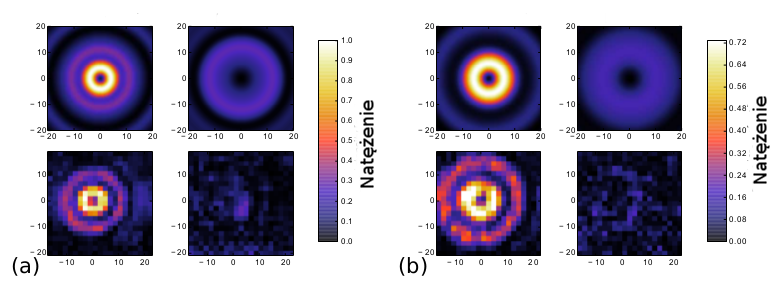
\includegraphics[width=\textwidth]{images/thz/exp-express.png}
	\caption{Przekroje natężenia wiązki w odległości (a) 80 mm i (b) 110 mm od soczewki uzyskane dla kierunku przepuszczającego (z lewej strony) oraz blokującego (z prawej strony). Rysunki w górnym rzędzie prezentują wyniki symulacji uzyskanych metodą BOR-FDTD, dolne zostały uzyskane eksperymentalnie. Odległości na rysnukach oznaczono w mm. Natężenie przedstawiono w jednostkach umownych~\cite{Yavorskiy:14}.}
	\label{fig:eksp-por}
\end{figure}




\chapter{\mbox{Absorbery} \mbox{elektromagnetyczne} \mbox{o~budowie} \mbox{warstwowej}}
\label{roz:pml}
Absorbery elektromagnetyczne znajdują zastosowania m. in. w budowie detektorów, fotowoltaice oraz kolorowaniu plazmonicznym. Niniejszy rozdział zawiera propozycję wykorzystania teorii ośrodków efektywnych do projektowania absorberów o~konstrukcji warstwowej. W oparciu o podobną postać tensora przenikalności elektrycznej materiału UPML~(ang. uniaxial perfectly matched layer; por. rozdział~\ref{art:pml}) i efektywnego tensora przenikalności elektrycznej struktury warstwowej~(patrz podrozdział \ref{subart:effmedium}) możliwe jest, w ograniczonym stopniu, odzwierciedlenie własności materiału UPML za pomocą struktury warstwowej. Początek rozdziału stanowi wprowadzenie do tematyki absorberów. W~dalszej części przedstawione zostało wyprowadzenie absorbera numerycznego UPML za pomocą optyki transformacyjnej~\cite{pendry2012transformation}. W kolejnym podrozdziale zaprezentowano możliwość realizacji metamateriału o~własnościach efektywnych odpowiadających warstwie UPML za pomocą wielowarstwy~\cite{ania2015}. Zaproponowano również wielowarstwę opartą o~dostępne materiały, wykazującą własności nieodbijającej warstwy absorpcyjnej dla długości fali $8$~µm.



\section{Powłoki antyodbiciowe i absorbery}
\subsection{Warstwa antyrefleksyjna}
\begin{figure}[tb]
	\centering
        \begin{subfigure}{0.42\textwidth}
		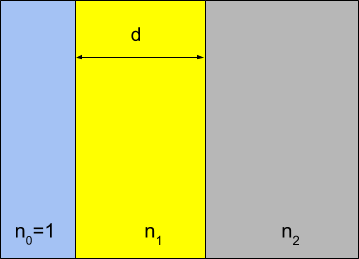
\includegraphics[width=\textwidth]{images/pml/antiref.png}
                \caption{}
		\label{fig:antyref}
        \end{subfigure}
        \begin{subfigure}{0.47\textwidth}
                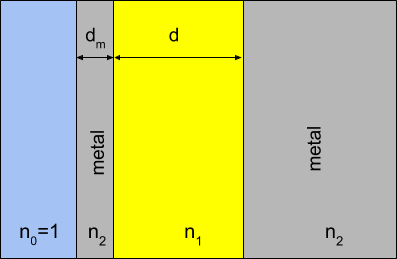
\includegraphics[width=\textwidth]{images/pml/sailsbury.png}
                \caption{}
		\label{fig:sailsburyschem}
        \end{subfigure}
        \caption{(a) Schemat prostej warstwy antyodbiciowej  (b) Płytka absorbująca Salisburego}
\end{figure}



\begin{figure}[tb]
	\centering
	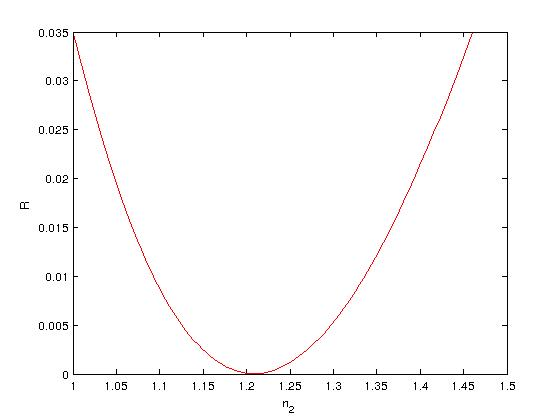
\includegraphics[width=\textwidth]{images/antyref.jpg}
	\caption{Zależność współczynnika odbicia od współczynnika załamania warstwy antyrefleksyjnej dla warstwy o grubości $d=\frac{\lambda_0}{4 n_1}$ umieszczonej pomiędzy powietrzem o $n_0=1$, a materiałem o współczynniku załamania $n_2=1.5$}
	\label{fig:antyref-result}
\end{figure}


Działanie prostych absorberów elektromagnetycznych jest analogiczne do warstwy antyodbiciowej. Rozważmy   warstwę antyodbiciową przedstawioną na rysunku \ref{fig:antyref}. Na granicy powietrza i dielektryka o współczynniku załamania $n_2$ wprowadziliśmy inny dielektryk o współczynniku załamania $n_1$, takim że $1<n_1<n_2$. Dokładne wartości współczynnika odbicia od obu granic ośrodków możemy obliczyć za pomocą równań Fresnela. Dla prostoty skupmy się na szczególnym przypadku padania normalnego. Natężeniowy współczynnik odbicia od granicy powietrza i ośrodka o współczynniku załamania $n_2$ wynosi:
\begin{equation}
R=\bigg|\frac{1-n_2}{1+n_2}\bigg|^2.
\end{equation}
Jeżeli jednak pomiędzy powietrze i dielektryk wprowadzimy dodatkową warstwę, wtedy natężeniowy współczynnik odbicia od takiego układu wyraża się wzorem
\begin{equation}
R=\Bigg| \frac{r+r' exp(2 i\phi)}{1+r r' exp(2 i\phi)} \Bigg|^2,
\end{equation}
w którym $r$ i $r'$ oznaczają odpowiednie amplitudowe współczynniki odbicia od granicy ośrodków wynikające z wzorów Fresnela:
\begin{equation}
r=\frac{1-n_1}{1+n_1},
\end{equation}
\begin{equation}
r'=\frac{n_1-n_2}{n_1+n_2},
\end{equation}
a $\phi$ oznacza zmianę fazy fali E-M w trakcie propagacji przez dodatkową warstwę $\phi=k_0 d n_1$, gdzie $d$ to grubość warstwy, $k_0$ to długość wektora falowego w próżni, a $k_y$ to długość wektora falowego w kierunku równoległym do granicy warstw.

 W ten sposób uzyskaliśmy układ dla którego współczynnik odbicia jest mniejszy niż współczynnik odbicia od materiału, ściśle półprzestrzeni wypełnionej materiałem, o współczynniku załamania $n_2$. Zależność współczynnika odbicia od układu z warstwą antyrefleksyjną w zależności od współczynnika załamania $n_1$ dla $n_2=1.46$ przedstawia wykres na rysunku \ref{fig:antyref-result}. Współczynnik odbicia przyjmuje zerową wartość dla $n_1=\sqrt{n_0 n_2}$.

Podstawowym mechanizmem, wykorzystywanym w konstrukcji warstw antyodbiciowych jest interferencja. Dobranie grubości $d=\frac{\lambda_0}{4 n_1}$, gdzie $\lambda_0$ to długość fali w próżni, prowadzi do destruktywnej interferencji między falami odbitymi od pierwszej i drugiej granicy ośrodków. Prowadząc do $R=0$ dla długości fali $\lambda_0$. Powstałe w ten sposób minimum współczynnika odbicia $R=0$, występuje dla wąskiego zakresu długości fali. Możliwe jest uzyskanie niskiego współczynnika odbicia dla szerokiego zakresu długości fali poprzez dodanie kolejnych warstw, o innej grubości optycznej. Współczynniki załamania w tak zbudowanej strukturze muszą zmieniać się zgodnie z postępem geometrycznym $n_i^2=n_{i-1} \cdot n_{i+1}$, a grubość każdej z warstw musi spełniać warunek $d_i=\frac{\lambda_0}{4 n_i}$  Projektując takie struktury możliwe jest uzyskiwanie powierzchni o wybiórczym, ze względu na częstotliwość, współczynniku odbicia~\cite{monacelli2005infrared}. 

\subsection{Ekran Salisbury'ego}
Również na zasadzie interferencyjnego wygaszenia odbicia, działa prosty absorber przedstawiony na rysunku \ref{fig:sailsburyschem}. Przed zwierciadłem w odległości $d$ znajduje się cienka warstwa metalu. Grubość warstwy $d_m$ musi być porównywalna z grubością naskórkową, aby umożliwić transmisję fal E-M przez tę warstwę. W ten sposób pomiędzy zwierciadłem, a cienką warstwą o grubości $d_m$ powstaje wnęka rezonansowa. Zazwyczaj tłumienie wprowadza się za pomocą urojonej części przenikalności $n_1$, możliwe jest jednak oparcie tłumienia jedynie na stratach związanych z grubą warstwą metalową tworzącą zwierciadło. 

\begin{figure}[tb]
	\centering
	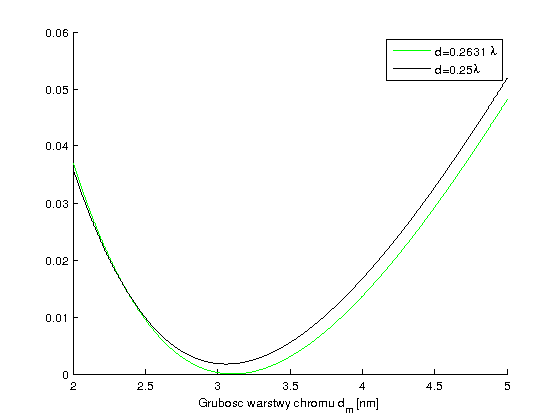
\includegraphics[width=\textwidth]{images/pml/sailsbury-res.png}
	\caption{Zależność natężeniowego współczynnika odbicia od grubości warstwy metalowej $d_m$, dla grubości warstwy o współczynniku załamania $n_2=3.34 + 4.27i$ równiej odpowiednio $d=0.2631\lambda_0$ i $d=0.25\lambda_0$}
	\label{fig:sailsburyres}
\end{figure}

Jako przykład,  wykres na rysunku \ref{fig:sailsburyres}  przedstawia zależność współczynnika odbicia od układu przedstawionego na rysunku \ref{fig:sailsburyschem} dla padającego promieniowania o długości fali $\lambda_0$=633~nm w zależności od $d_m$. Jako współczynnik załamania w cienkiej warstwie metalowej przyjęto $n_2=3.34+4.27i$ co odpowiada własnościom chromu dla rozważanej długości fali~\cite{ordal1983optical}. Dobranie odpowiedniej odległości $d$ i grubości warstwy chromu $d_m$ pozwala na wytworzenie warunków destruktywnej interferencji umożliwiając uzyskanie zerowego współczynnika odbicia. W wyniku odbicia na granicy ośrodków o współczynnikach załamania $n_1$ i $n_2$ wprowadzane jest również przesunięcie fazy. Konieczność skompensowania tego przesunięcia, jak i skończone rozmiary warstwy półprzepuszczalnej $d_m$ powodują, że optymalna grubość materiału o współczynniku załamania $n_1$ nieco odbiegają od $\frac{\lambda_0}{4 n_1}$, co ilustrują wyniki na rysunku \ref{fig:sailsburyres}. 

\subsection{Inne propozycje realizacji absorberów}

Innym podejściem jakie można spotkać w literaturze jest wytworzenie warstw nie odbijających za pomocą cienkiej warstwy ferro- i ferimagnetyków tworzących  statyczną magnetyzację o charakterze periodycznym   \cite{ramprecht2008scattering}. Autorzy prezentują wyniki symulacji dowodzące możliwości uzyskania współczynnika odbicia poniżej -20dB w~zakresie od 1 do 4 GHz, niezależnie od kąta padania. W~ostatnich latach proponowane były również absorbery oparte na rezonatorach SRR~(ang.~split-ring resonator), w których warstwa nieodbijająca jest realizowana poprzez uzyskanie dopasowania impedancyjnego z powietrzem jednocześnie wykorzystują stratność w metamateriale. Omówienie prac wykorzystujących tę technikę  można znaleźć w~artykule~\cite{watts2012metamaterial}.

Imponujące wyniki eksperymentalne pozwalające uzyskać wysoki współczynnik absorpcji w szerokim zakresie spektralnym zostały uzyskane za pomocą lasów nanorurek węglowych \cite{mizuno2009black}. Zaprezentowane przez autorów wyniki eksperymentalne wskazują na współczynnik odbicia mniejszy niż 2\% w zakresie od 200~nm do 20µm.

Możliwa jest również konstrukcja absorberów opartych o wielowarstwy metaliczno-dielektryczne. Tego typu absorbery osiągają współczynnik absorpcji większy niż 80\%, dla całego zakresu długości fali ciała doskonale czarnego o temperaturze 300K~\cite{guo2014impact,corrigan2012broadband}. Autorzy dyskutują w pracy dalsze możliwości zmniejszenia współczynnika odbicia poprzez wprowadzenie dodatkowej porowatej warstwy antyodbiciowej. 

W kolejnych podrozdziałach przedstawiona zostanie inna możliwa do zastosowania koncepcja umożliwiająca uzyskanie warstwy charakteryzującej się niskim współczynnikiem odbicia w szerokim zakresie długości fali i kątów padania. 

\section{Wyprowadzenie UPML~(ang. uniaxial perfectly matched layer)}
Rozważania dotyczące PML zacznijmy od przytoczenia ogólnej postaci równania falowego~\cite{barton1989elements}
\begin{equation}
\nabla \cdot ( a \nabla U) = \frac{1}{b} \frac{\partial^2 u}{\partial t^2} = \frac{\ddot{u}}{b},
\label{eq:wave}
\end{equation}
gdzie przez $u(\vec{x},t)$ oznaczono skalarną amplitudę fali, $a=a(\vec{x})$ i~$b=b(\vec{x})$ są parametrami, które opisują ośrodek w~którym propaguje się fala. Dla tak sformułowanego równania, możemy zdefiniować wielkość $c=\sqrt{ab}$ mającą interpretację prędkości fazowej fali opisywanej powyższym równaniem. Równanie (\ref{eq:wave}) jest równaniem różniczkowym drugiego rzędu, które możemy zapisać w~postaci układu dwóch równań z~pierwszą pochodną poprzez wprowadzenie pola $\vec{v}(x,t)$:
\begin{equation}
\frac{\partial u}{\partial t} = b \nabla \cdot \vec{v},
\end{equation}

\begin{equation}
\frac{\partial \vec{v}}{\partial t}= a\nabla u.
\end{equation}
Powyższe dwa równania, możemy zapisać  w~postaci równania wektorowego
\begin{equation}
\frac{\partial \vec{w}}{\partial t}=\frac{\partial}{\partial t} {u \choose \vec{v}} = 
	\begin{pmatrix}
		& b\nabla\cdot \\
	a\nabla & \\
	\end{pmatrix}
{u \choose \vec{v}} = \hat{D}\vec{w},
\label{eq:gen-wave-eq}
\end{equation}
dla liniowego operatora $\hat{D}$ i~$\vec{w}=(u;\vec{v})$ ( dla $\vec{v}$ należącego do przestrzeni trójwymiarowej $\vec{w}$ jest czterowektorem). Kluczową własnością, która decyduje o~tym, że równanie~(\ref{eq:gen-wave-eq}) jest ,,równaniem falowym''  okazuje się być antyhermitowskość operatora $\hat{D}$\footnote{Macierz nazywamy antyhermitowską wtedy gdy spełnia warunek $A$=-$A^\dag$, gdzie przez $^\dag$ rozumiemy sprzężenie hermitowskie macierzy, równoważne dokonaniu transpozycji i~sprzężenia zespolonego wszystkich elementów macierzy.}. To właśnie z~tej własności wynikają oscylujące rozwiązania równania, oraz spełnienie prawa zachowania energii mające kluczowe znaczenie dla fizyki fal. Każde równanie falowe, zaczynając od równań skalarnych, przez równania Maxwella,  po równanie Schr\"{o}dingera i~równania Lam\'{e}-Navier'a~(opisującego fale sprężyste w~ciałach stałych) może zostać przedstawione w~formie $ \frac{\partial  \vec{w}}{\partial t}=\hat{D}\vec{w}$, dla pewnej funkcji falowej $\vec{w}$ i~antyhermitowskiego operatora $\hat{D}$~\cite{johnson2007notes}. W niniejszej pracy skupiamy się na zastosowaniu PML w~elektromagnetyzmie, te same koncepcje mogą być jednak zastosowane do wszystkich wymienianych przypadków.

Załóżmy, że $w(x,t)$ jest rozwiązaniem równania falowego w~nieograniczonej przestrzeni. Interesujące nas zjawiska zachodzą w~okolicy początku układu współrzędnych $x=0$, a obszar symulacji chcemy zakończyć tak, aby absorbował fale propagujące się. W szczególności skupimy się na zakończeniu obszaru symulacji dla dodatniej części osi $+x$ (rozważanie dla pozostałych kierunków jest analogiczne). Zakończenie obszaru symulacji przeprowadzimy w~czterech krokach:
\begin{enumerate}
	\item W nieskończonej przestrzeni wykonamy analityczne przedłużenie równania falowego i~rozwiązania do zespolonego konturu $\tilde{x}$.
	\item Dla konturu $\tilde{x}$ nie będącego konturem czysto rzeczywistym, fale propagujące się poza interesującym nas obszarem zmieniane są na fale zanikające bez wprowadzenia odbicia.
	\item W nieograniczonej przestrzeni wykorzystamy optykę transformacyjną,  tak aby wyrazić zespolony $\tilde{x}$ przez rzeczywiste położenie. W nowych współrzędnych otrzymamy rzeczywiste położenia i~materiały których własności są opisywane za pomocą liczb zespolonych.
	\item Zakończymy obszar symulacji w~obliczonym na podstawie zamiany zmiennych materiale w~miejscu w~którym pole będzie na tyle stłumione, aby zastosowany warunek brzegowy nie miał znaczenia.
\end{enumerate}

Zakładamy dalej, że przestrzeń znajdująca się daleko od interesującego nas obszaru w~okolicach $x=0$, jest jednorodna, liniowa i~nie zmienia się w~zależności od czasu. Dzięki tym założeniom, fala propagująca się musi przyjmować formę superpozycji fal płaskich:
\begin{equation}
	w(\vec{x},t)= \sum_{\vec{k},\omega} W_{\vec{k},\omega} e^{i (k_x x-\omega t)},
	\label{eq:pml-cos}
\end{equation}
gdzie $W_{\vec{k},\omega}$ są jedynie funkcjami położenia, $\omega$ częstością kołową, a $\vec{k}$ wektorem falowym dla fali w~ośrodku izotropowym z~zależnością dyspersyjną $\omega=c k_0$, gdzie $c$ oznacza prędkość fazową. Dla fal propagujących się w~kierunku $+x$ prędkość grupowa $\frac{d \omega}{d k}$ jest dodatnia. Kierunek prędkości fazowej i~grupowej w~ośrodkach jednorodnych są zgodne z~wyjątkiem kilku szczególnych przypadków~\cite{teixeira1998general}. Dlatego dalej założymy, że $k_x$ jest dodatnie. 

\begin{figure}[tb]
	\begin{subfigure}{0.45\textwidth}
		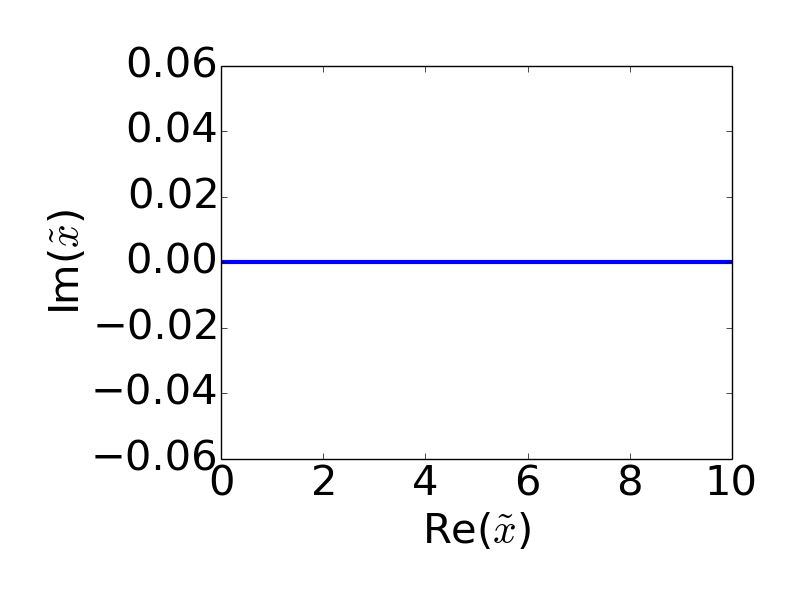
\includegraphics[width=\textwidth]{images/pml/real-x.png}
		\caption{}
	\end{subfigure}
	\begin{subfigure}{0.45\textwidth}
		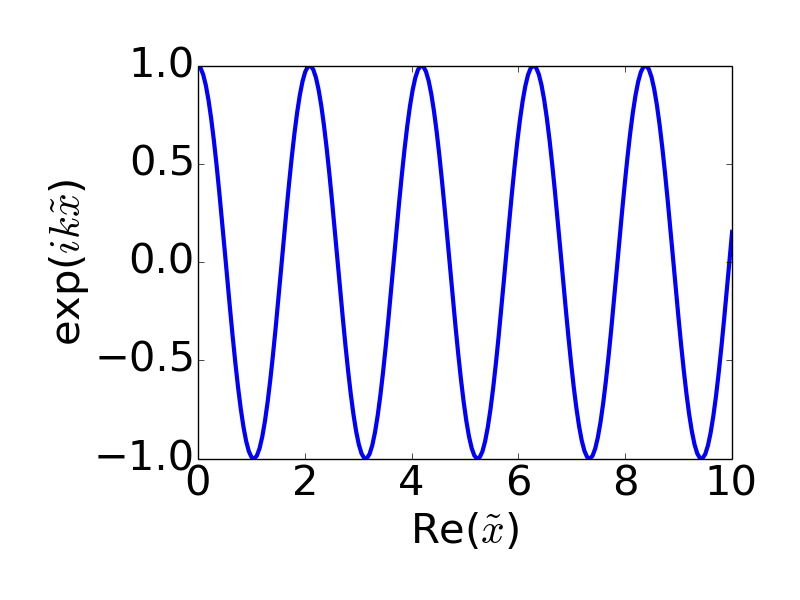
\includegraphics[width=\textwidth]{images/pml/real-x-wave.png}
		\caption{}
	\end{subfigure}


	\begin{subfigure}{0.45\textwidth}
		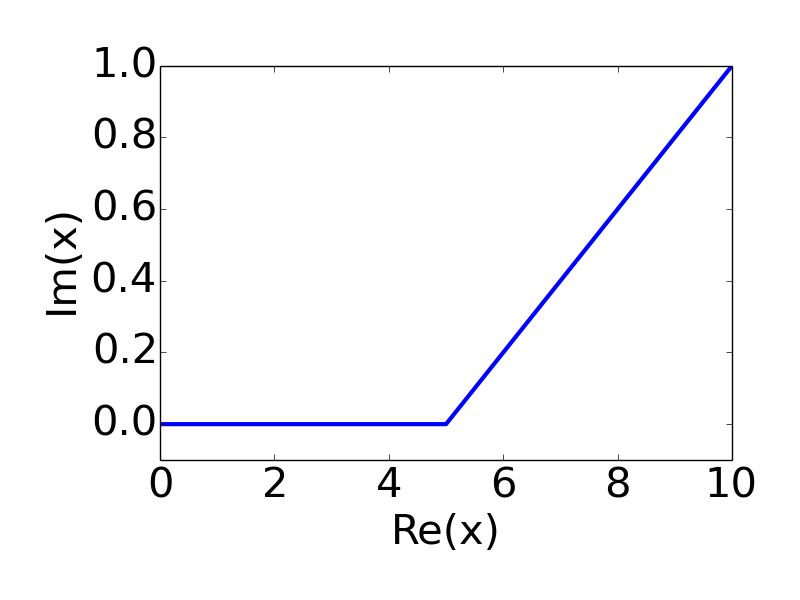
\includegraphics[width=\textwidth]{images/pml/complex-x.png}
		\caption{}
		\label{fig:complex-contour}
	\end{subfigure}
	\begin{subfigure}{0.45\textwidth}
		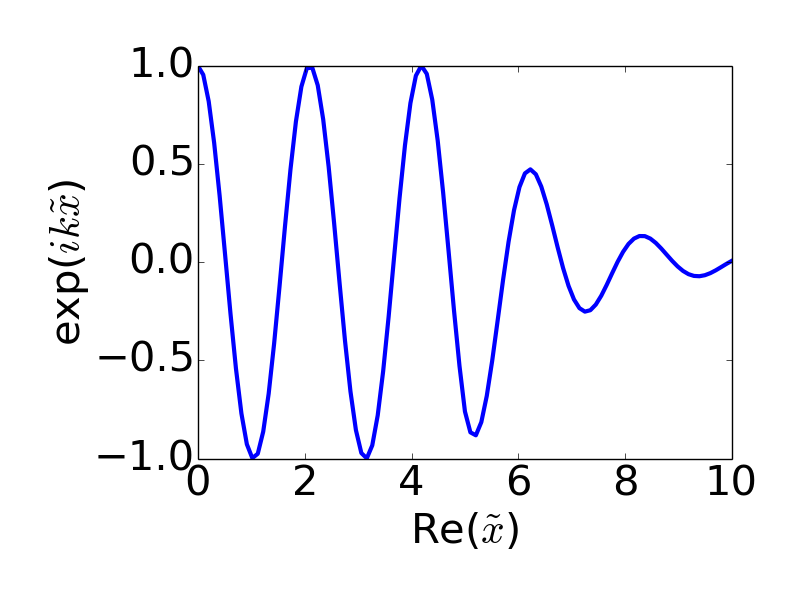
\includegraphics[width=\textwidth]{images/pml/complex-x-wave.png}
		\caption{}
		\label{fig:absorbing-region}
	\end{subfigure}

	\caption{Na rysunkach (a) i~(b) przedstawiono odpowiednio rzeczywiste wartości położenia na zespolonej płaszczyźnie $\tilde{x}$ i~odpowiadające im rozwiązanie równania falowego. Na rysunku (c) dla arbitralnej  wartości $\textrm{Re}(x)>5$ przedstawiono zmieniony kontur wykorzystujący zespolone wartości dla $\tilde{x}$. Odpowiednie dla zmodyfikowanego konturu (c)  rozwiązanie równania falowego przedstawia wykres na rysunku (d).}
	\label{fig:var-transform}
\end{figure}


Kluczowym jest zauważenie, że składniki sumy z wzoru (\ref{eq:pml-cos}) mogą zostać zapisane w~postaci
\begin{equation}
\vec{W}(y,z)e^{i(k\tilde{x}-\omega t)},
\end{equation}
która to jest funkcją analityczną w~$\tilde{x}\in \mathbb{C}$. Oznacza to, że możemy dokonać jej analitycznego przedłużenia dla zespolonych wartości $x$. Falę propagującą, wraz z~czysto rzeczywistym konturem opisującym położenia w~kierunku $x$ przedstawiają wykresy na rysunku \ref{fig:var-transform}a i~\ref{fig:var-transform}b. 

Dla lepszego zrozumienia koncepcji rozważmy teraz zamianę zmiennych dla obszaru $x>x_0$, w taki sposób, że: 
\begin{equation}
\tilde{x}=  
\begin{cases} 
        x, & \mbox{dla } x< x_0 \\ 
        x+0.2x\mbox{ }i, & \mbox{dla } x>x_0 \\
\end{cases}.
\end{equation}
Rozwiązanie zagadnienia propagacji po takim zespolonym konturze dla $x_0=5$ przedstawia wykres na rysunku \ref{fig:complex-contour}. Zauważymy, że dla obszaru w~którym do rzeczywistej części dodaliśmy liniowo rosnącą część urojoną uzyskujemy falę zanikającą. Ponieważ na wykresie \ref{fig:absorbing-region} rozwiązanie dla $x<x_0$ nie uległo zmianie, a w~obszarze $x>x_0$ obserwujemy fale zanikającą to przestrzeń dla $x>x_0$ wykazuje działanie nieodbijającej warstwy absorpcyjnej.

Zgodnie z przedstawionym przykładem rozwinięcie analityczne możemy dla wygody obliczeniowej traktować równoważnie z~zamianą współrzędnych w~omawianym równaniu różniczkowym. Oznaczmy zespoloną zmienną $\tilde{x}(x)=x+if(x)$, traktując od tej pory $x$ zawsze jako rzeczywiste położenie. Taka zamiana współrzędnych wymaga od nas zamiany każdego różniczkowania po zdeformowanym konturze $\partial \tilde{x} = (1+i\frac{df}{dx}) \partial x$. Ponieważ założyliśmy, że nasze równanie różniczkowe jest niezależne od x (przynajmniej dla dużych x, gdzie $f(x)\ne0$; wynika to bezpośrednio z~założenia jednorodności liniowości i~niezależności od czasu) nie musimy uwzględniać żadnych dodatkowych wyrazów. Jak wykażemy w~kolejnych akapitach wygodnie jest wybrać $\frac{df}{dx}=\frac{\sigma_x}{\omega}$ i~ostatecznie zapisać wymaganą zamianę zmiennych jako:
\begin{equation}
	\frac{\partial}{\partial \tilde{x}} \to \frac{1} {1+i \frac{\sigma_x(x)}{\omega}} \frac{\partial}{\partial x}.
	\label{eq:pml-variable-change}
\end{equation}

W obszarach PML, gdzie $\sigma_x\ne0$, oscylujące rozwiązania równania falowego przyjmują postać fal eksponencjalnie zanikających. Poza PML ( $\sigma_x=0$) rozwiązywane równanie pozostaje niezmienione: nie występują odbicia ponieważ jest to analityczne rozwinięcie pierwotnego rozwiązania i~w obszarach gdzie $\tilde{x}=x$ rozwiązanie nie może się zmienić.

Po wykonaniu podstawienia (\ref{eq:pml-variable-change}), rozwiązania równania falowego w~obszarze PML przyjmują postać:
\begin{equation}
e^{ikx}\textrm{exp}\Big(-\frac{k}{\omega}\int^x \sigma_x(x')dx'\Big).
\end{equation}
Warto zauważyć, że pojawiający się wykładnik potęgi $\frac{k}{\omega}$ dla materiałów bezdyspersyjnych jest stały i~równy odwrotności prędkości fazowej. W ten sposób uzasadniliśmy zaproponowany wybór $\frac{df}{dx}=\frac{\sigma_x}{\omega}$, dzięki któremu otrzymujemy niezależność współczynnika tłumienia od częstotliwości promieniowania E-M. 

Zasadniczo zgodnie z~przedstawionym wyprowadzeniem możemy zastosować dowolnie mały obszar PML, ponieważ nie ma żadnego ograniczenia na wartości $\sigma_x$. W praktyce numerycznej, ze względu na zastosowaną dyskretyzację gwałtowne zmiany $\sigma_x$ prowadzą do powstania ,,odbić numerycznych''. Z tego powodu $\sigma_x$ zazwyczaj ma postać funkcji kwadratowej lub sześciennej narastającej od zera do wartości maksymalnej na obszarze większym od połowy długości fali promieniowania występującego w~symulacji~\cite{johnson2008notes}.

W przypadku równań Maxwella każda zamiana współrzędnych może zostać wyrażona przez równania Maxwella we współrzędnych kartezjańskich ze zmienionymi materiałami~\cite{ward1996refraction}. Zamiana współrzędnych jest równoważna zmianie przenikalności elektrycznej $\varepsilon$ i~magnetycznej $\mu$, w~ogólności na absorbujące ośrodki anizotropowe. 

W przypadku trójwymiarowych równań Maxwella dla ośrodka opisywanego za pomocą tensorów $\hat{\varepsilon}$ i~$\hat{\mu}$ 
\begin{equation}
\hat{\varepsilon}=
\begin{bmatrix}
\varepsilon_x & 0 & 0 \\
0 &\varepsilon_y & 0 \\
0 & 0  & \varepsilon_z  \\
\end{bmatrix}
, \hat{\mu}=
\begin{bmatrix}
\mu_x & 0 & 0 \\
0 &\mu_y & 0 \\
0 & 0  & \mu_z  \\
\end{bmatrix}
\end{equation}
warstwą PML może być materiał charakteryzujący się przenikalnością elektryczną i~magnetyczną opisywaną tensorami:
\begin{equation}
\hat{\varepsilon}_{\textrm{PML}}=
\begin{bmatrix}
s \cdot \varepsilon_x & 0 & 0 \\
0 &s \cdot \varepsilon_y & 0 \\
0 & 0  & \frac{ \varepsilon_z}{s}  \\
\end{bmatrix}
, \hat{\mu}_{\textrm{PML}}=
\begin{bmatrix}
s \cdot \mu_x & 0 & 0 \\
0 & s \cdot \mu_y & 0 \\
0 & 0  & \frac{\mu_z}{s}  \\
\end{bmatrix},
\label{eq:general-pml-form}
\end{equation}
gdzie $s$ jest dowolną liczbą zespoloną~\cite{sacks1995perfectly}, której część odpowiedzialna za tłumienie jest równoznaczna liniowemu współczynnikowi deformacji konturu zmiennych przestrzennych w~część urojoną.



\section{Realizacja PML za pomocą struktury warstwowej}
\begin{figure}[tb]
	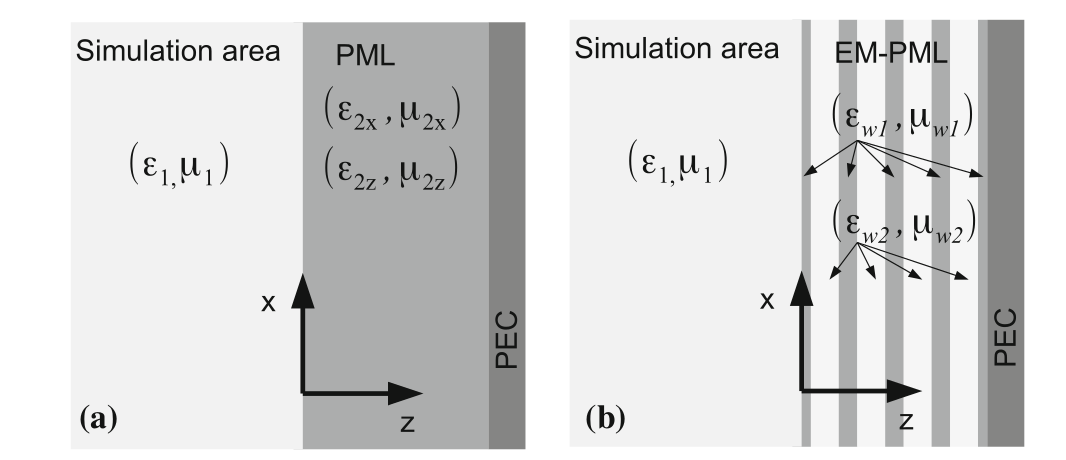
\includegraphics[width=\textwidth]{images/pml/oqe_schemat.png}
	\caption{Schematyczne przedstawienie analizowanej struktury warstwowej i~przybliżanego za pomocą modelu ośrodka efektywnego ośrodka PML}
	\label{fig:pml-multilay-schem}
\end{figure}

Porównując ogólną postać PML podaną w~równaniu (\ref{eq:general-pml-form}) z~modelem ośrodka efektywnego przedstawionym w~podrozdziale \ref{subart:effmedium} można zaproponować przybliżenie ośrodka typu PML za pomocą struktury warstwowej o~odpowiednich właściwościach efektywnych. Schematycznie taką wielowarstwę przedstawia rysunek \ref{fig:pml-multilay-schem}. W szczególności, dla uproszczenia analizy, skupimy się na polaryzacji TM, dla której istotnymi składowymi tensorów opisujących własności materiałowe są:~$\varepsilon_x$~,$\mu_y$~i $\varepsilon_z$. Ze względu na ograniczenia używanego modelu ośrodka efektywnego, zgodnie ze schematem na rysunku \ref{fig:pml-multilay-schem} otrzymujemy $\varepsilon_x=\varepsilon_y$, oraz $\mu_x=\mu_y$. Ponownie odwołując się do granicy między ośrodkami na rysunku \ref{fig:pml-multilay-schem}a, otrzymujemy warunki dla których wielowarstwa złożona z~materiałów $w1$ i~$w2$ schematycznie przedstawiona na rysunku \ref{fig:pml-multilay-schem}b będzie efektywnie spełniać rolę PML pod warunkiem spełnienia następujących równości:
\begin{equation}
	f\cdot \varepsilon_{w1} + (1-f)\cdot \varepsilon_{w2} = s \cdot \varepsilon_1,
	\label{eq:oqe4}
\end{equation}

\begin{equation}
	[f\cdot \varepsilon_{w1}^{-1}+(1-f)\varepsilon_{w2}^{-1}]^{-1}=s^{-1}\cdot \varepsilon_1,
	\label{eq:oqe5}
\end{equation}

\begin{equation}
	f\cdot \mu_{w1} + (1-f)\cdot \mu_{w2} = s \cdot \mu_1,
	\label{eq:oqe6}
\end{equation}
gdzie przez $f$ oznaczony został współczynnik wypełnienia, równy ułamkowi przestrzeni wielowarstwy zajmowanemu przez materiał $w1$. Odpowiednie warunki dla polaryzacji TE to:
\begin{equation}
	\varepsilon_{w1}=\rho \frac{\varepsilon_1 \cdot s}{f\cdot \rho + (1 -f) },
	\label{eq:te-eps1}
\end{equation}

\begin{equation}
	\varepsilon_{w2}=\frac{\varepsilon_1 \cdot s}{f\cdot \rho + (1-f)},
	\label{eq:te-eps2}
\end{equation}
gdzie
\begin{equation}
	\rho = 1+\frac{s^2-1 \pm \sqrt{(s^2-1)(s^2-(2f-1)^2)}}{2f(1-f)}.
	\label{eq:te-rho}
\end{equation}

\begin{figure}[tb]
	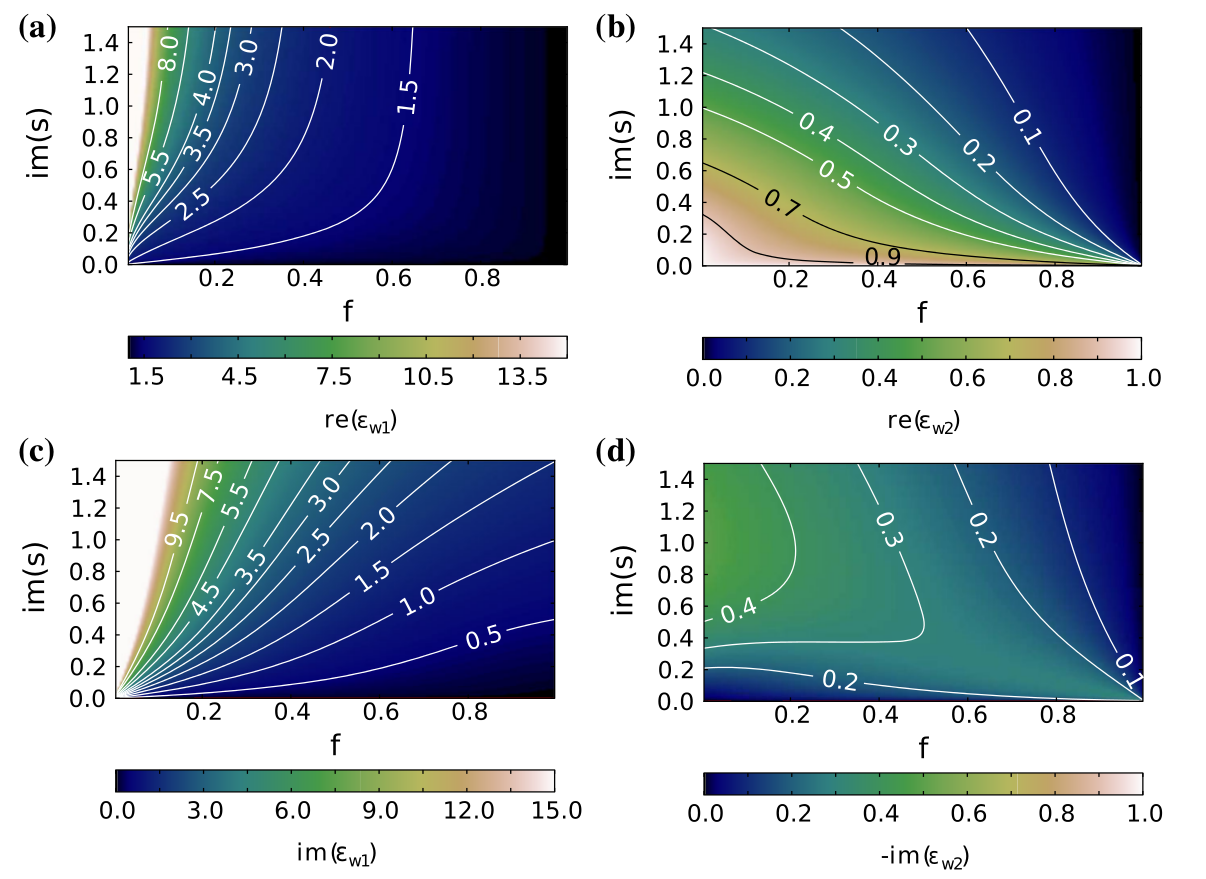
\includegraphics[width=\textwidth]{images/pml/oqe_materials.png}
	\caption{Zależność przenikalności elektrycznej materiałów tworzących UPML (w lewej kolumnie $\varepsilon_{w1}$, w~prawej $\varepsilon_{w2}$) w~funkcji współczynnika wypełnienia i~urojonej części parametru $s$ (założono, że $\textrm{Re}(s)$=1. Górny wiersz na wykresach (a) i~(b) prezentuje zależności części rzeczywistych, dolny na wykresach (c) i~(d) części urojonych przenikalności elektrycznych. Ujemne wartości $\varepsilon$ na wykresach (c) i~(d) odpowiadają materiałom ze wzmocnieniem optycznym. }
	\label{fig:upml-eps-s-f}
\end{figure}

Wykresy na rysunku \ref{fig:upml-eps-s-f} prezentują wyniki obliczonych zgodnie z~(\ref{eq:te-eps1}) i~(\ref{eq:te-eps2}) wartości $\varepsilon_{w1}$ i~$\varepsilon_{w2}$ jako funkcje współczynnika wypełnienia $f$ i~parametru $s$, dla którego przyjęto $s=1+\alpha i$. Używamy rozwiązań dla (\ref{eq:te-rho}) z~$|\rho|>1$. Podobne wyrażenia jak (\ref{eq:oqe4}) i~(\ref{eq:oqe5}) można wypisać i~rozwiązać dla $\mu_{w1}$ i~$\mu_{s2}$. W przypadku gdy $\varepsilon_1=\mu_1$ otrzymujemy $\varepsilon_{w1}=\mu_{w1}$ i~$\varepsilon_{w2}=\mu_{w2}$. Należy podkreślić, że dla każdej pary $f$ i~$s$ przedstawionej na wykresach \ref{fig:upml-eps-s-f} uzyskujemy metamateriał, który w~omawianym przybliżeniu będzie spełniał funkcje UPML, dla każdej pary $f$ i~$s$ potrzebujemy jednak wybrać inne materiały $w1$ i~$w2$.

W kolejnym kroku możemy obliczyć natężeniowy współczynnik odbicia od struktury zaprezentowanej na rysunku \ref{fig:pml-multilay-schem}b dla $f=0.6$, oraz $\textrm{Im}(s)=$0.5 lub $\textrm{Im}(s)=$5. Zależność współczynnika odbicia od kąta padania, oraz grubości komórki elementarnej wielowarstwy przedstawia wykres na rysunku \ref{fig:oqe3}. Ze względu na umieszczenie idealnego przewodnika za wielowarstwą współczynnik odbicia łączy w~sobie część odbijaną od wielowarstwy, jak i~transmitowaną przez wielowarstwę i~odbijaną od zwierciadła z~PEC~(ang. perfect electric conductor) . Analizując wykres \ref{fig:oqe3} możemy zauważyć, że wraz ze wzrostem $\frac{a}{\lambda}$ zmniejsza się współczynnik odbicia fal propagujących się, którym odpowiada część wykresu, dla którego na osi odciętych wartości spełniają nierówność $\frac{k_x}{k_0}<1$.

Wynika to ze zwiększania grubości warstwy pochłaniającej, więc jest przede wszystkim związane ze zmniejszeniem transmisji przez wielowarstwę, a nie zmianą odbicia od pierwszej granicy warstw. W przypadku fal ewanescentnych $\frac{k_x}{k_0}>1$, obserwujemy wzrost współczynnika odbicia. Można to interpretować jako odbicie od pierwszej warstwy wynikające z~niespełnienia warunków homogenizacji (przybliżenie ośrodka efektywnego zakłada $\frac{a}{\lambda} <<$ 1) przez strukturę. Dlatego wzrost jest większy dla większej części urojonej współczynnika $s$, skutkującej większą różnicą współczynników załamania na granicy pierwszej warstwy i~powietrza.

\begin{figure}[tb]
	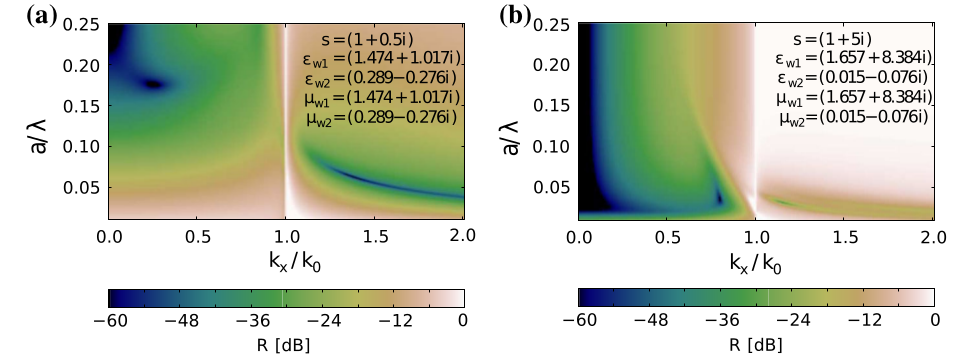
\includegraphics[width=\textwidth]{images/pml/fig3.png}
	\caption{Zależność natężeniowego współczynnika odbicia od kąta padania i~okresu wielowarstwy dla struktury zgodniej ze schematem na rysunku \ref{fig:pml-multilay-schem}, dla $N=5$ par warstw, przy współczynniku wypełnienia $f=0.6$. Rysunek po lewej (a) przedstawia wyniki dla $s=1+0.5i$, wykres po prawej przedstawia wyniki dla $s=1+5i$.}
	\label{fig:oqe3}
\end{figure}

Przedstawione wyniki możliwe są do osiągnięcia za pomocą materiałów wykazujących szczególne własności elektryczne i~magnetyczne. W szczególności obliczenia zakładały zespoloną przenikalność magnetyczną, oraz wzmocnienie optyczne. Dla $s=1+5i$ możliwe jest uzyskanie warstwy PML o~całkowitej grubości $5\cdot a \approx \frac{\lambda}{20}$ wykazującej natężeniowy współczynnik odbicia ok -30dB dla szerokiego zakresu kątów padających fal płaskich.

W przypadku oświetlenia wielowarstwy za pomocą polaryzacji TM jeden ze współczynników przenikalności magnetycznej może zostać ustalony w~sposób arbitralny. W szczególności możemy więc założyć $\mu_{w2}=1$, ponieważ większość materiałów spotykanych w~przyrodzie charakteryzuje się taką wartością dla częstotliwości optycznych. Drugą przenikalność magnetyczną możemy wyznaczyć za pomocą wzoru \ref{eq:oqe6}. Część rzeczywista $\textrm{Re}(\mu_{w1})=1$, a zależność części urojonej $\textrm{Im}(\mu_{w1})$ od części urojonej współczynnika $s$, oraz współczynnika wypełnienia przedstawia wykres \ref{fig:im-mu1}. Na podstawie przywołanego wykresu możemy zauważyć, że wysoki współczynnik wypełnienia, oraz wykorzystanie niskiej części urojonej $s$ skutkują niskimi wartościami $\textrm{Im}(\mu_{w1})$. Jest to dla nas istotne ponieważ korzystając z~materiałów występujących w naturze, będziemy zmuszeni przybliżyć tę wartość przez $0$.

\begin{SCfigure}
	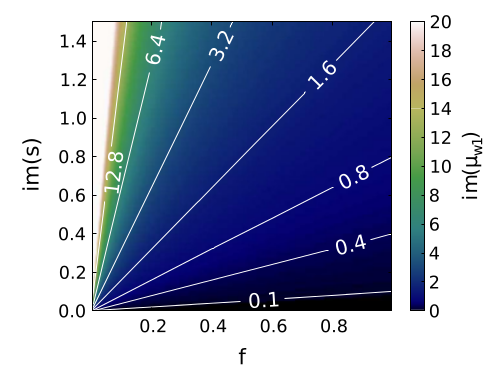
\includegraphics[width=0.6\textwidth]{images/pml/fig4.png}
	\caption{Zależność części urojonej przenikalności magnetycznej jednego z~materiałów $\mu_{w1}$, od części urojonej współczynnika $s$ i~współczynnika wypełnienia $f$ w~przypadku gdy założono $\mu_{w2}=1$}
	\label{fig:im-mu1}
\end{SCfigure}


W przypadku przygotowania eksperymentu, a nie np. wykorzystania do konstrukcji PML w~symulacjach  numerycznych, należy zaniedbać własności magnetyczne materiałów $\mu=1$, oraz zysk optyczny $\textrm{Im}(\varepsilon)\lt0$. Wyniki dla obu polaryzacji po zastosowaniu się do wymienionych przybliżeń przedstawiają wykresy na rysunku \ref{fig:pml-real-ref}. Zaproponowany absorber składa się z~materiału stratnego, oraz warstw charakteryzujących się przenikalnością elektryczną mniejszą od 1. Przedstawione wyniki obliczeń wskazują, że w~wyniku poczynionych założeń efektywność pracy wielowarstwy jako struktury PML znacznie różni się w~zależności od polaryzacji. W przeciwieństwie do obliczeń dla wielowarstw odpowiadających PML, narzucone warunki prowadzą do mniejszej wartości współczynnika odbicia dla polaryzacji TE. Wysokie współczynniki odbicia, uniemożliwiające zastosowanie wielowarstwy,  pojawiają się jednak jedynie dla kątów padania bliskich $90^{\circ}$, co jest charakterystyczne dla UPML.

\begin{figure}[tb]
	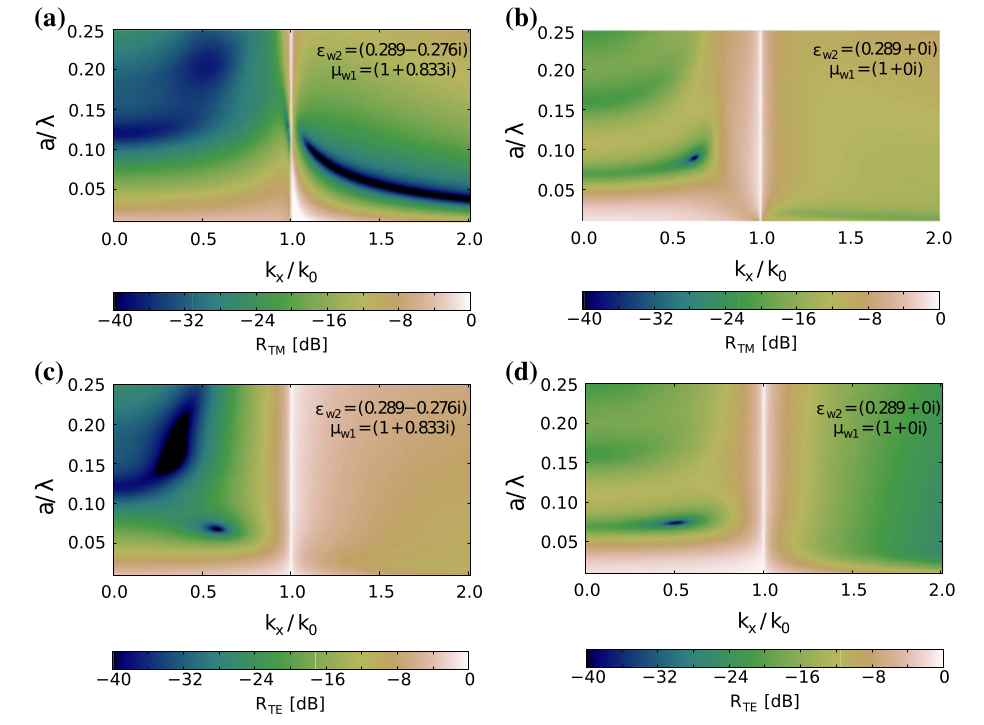
\includegraphics[width=\textwidth]{images/pml/fig5.png}
	\caption{Zależność natężeniowego współczynnika odbicia $R$, od kąta padania i~grubości warstw dla wielowarstwy składającej się z~$N=5$ okresów, dla $s=1+5i$ i~$f=0.6$. Spełniając założenie, że $\mu_{w2}=1$ (a,c), oraz $\mu_{w1}=\mu_{w2}=1$, $\textrm{Im}(\varepsilon_1)\ge 0 $ i~$\textrm{Im}(\varepsilon_2)\ge 0 $ (b,d). Wyniki dla polaryzacji TM (a,b) oraz TE (c,d). Przenikalność elektryczna $\varepsilon_{w1}=1.474+1.017i$.}
	\label{fig:pml-real-ref}
\end{figure}


Na podstawie przeprowadzonej dyskusji, można zaproponować prostą regułę jaką należy posługiwać się w~celu doboru materiałów do budowy wielowarstwy efektywnie przypominającej UPML graniczący z~powietrzem. Kluczowym elementem jest wykorzystanie materiału, którego część rzeczywista przenikalności elektrycznej znajduje się w~zakresie od 0 do 1. Przeprowadzone obliczenia wskazują również, że materiał ten powinien być możliwe bezstratny. Druga wykorzystywana substancja powinna posiadać część rzeczywistą przenikalności elektrycznej większą od 1, oraz wykazywać stratność. 

W ogólności w~szerokich zakresach spektralnych większość materiałów charakteryzuje się $\textrm{Re}(\varepsilon) > 1$. Wyjątkami są zakresy długości fali w~okolicach rezonansów dyspersyjnych (patrz. \ref{subart:lorenz-drude}). Możliwe jest również uzyskanie zaprojektowanych własności $\varepsilon$ w~metamateriałach np. w~strukturach funkcjonujących w~literaturze angielskojęzycznej pod nazwą \textit{fishnet}~\cite{valentine2008three}. 

Przykładem pary materiałów, które możemy zastosować w~realizacji UPML za pomocą wielowarstwy są $SiO_2$ i~$NaCl$ dla długości fali w~okolicach 8~$\mu$m. Przenikalności elektryczne zaproponowanych materiałów przedstawiają wykresy na rysunku \ref{fig:nacl-sio2-mat}. Rolę materiału o~przenikalności elektrycznej $\varepsilon \in (0,1)$, spełnia w~tym obszarze $SiO_2$, ponieważ dla długości fali $9.5$~$\mu$m występuje dla tego materiału rezonans. Również wartość efektywna części urojonej $\varepsilon$ wielowarstwy wynika głównie z~własności $SiO_2$. 

\begin{figure}[tb]
	\begin{subfigure}{0.45\textwidth}
		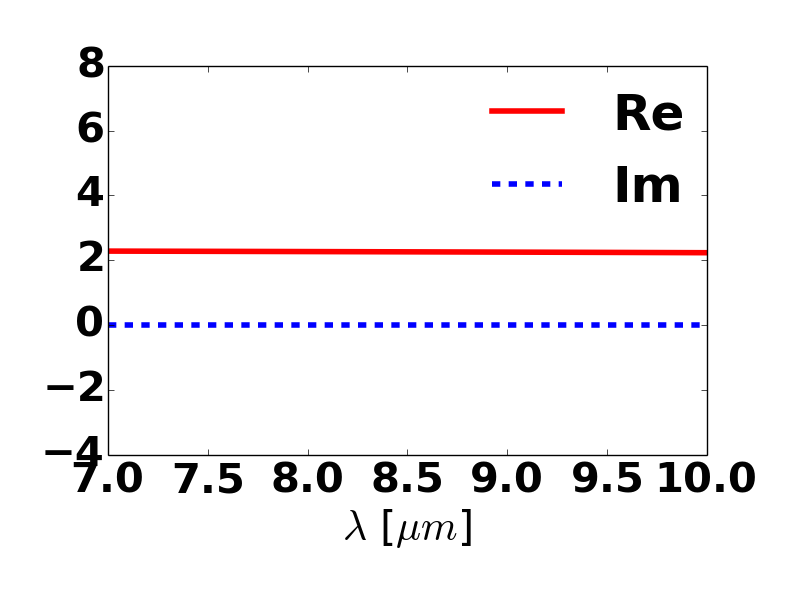
\includegraphics[width=\textwidth]{images/pml/nacl.png}
		\caption{}
	\end{subfigure}
	\begin{subfigure}{0.45\textwidth}
		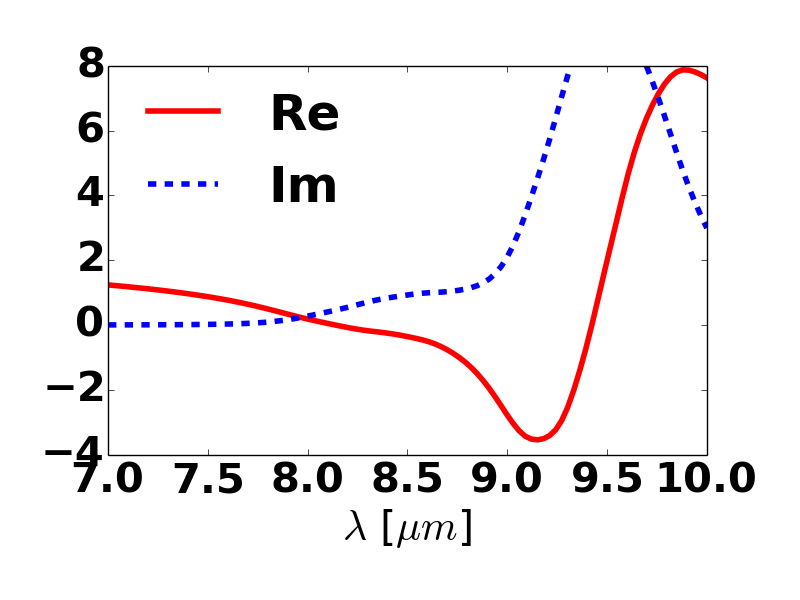
\includegraphics[width=\textwidth]{images/pml/sio2.png}	
		\caption{}
	\end{subfigure}
	\caption{Wartości przenikalności elektrycznej w~zakresie od 7 do 10~$\mu$m dla (a) $NaCl$~\cite{li1976refractive}, (b) $SiO_2$~\cite{Kischkat:12}}
	\label{fig:nacl-sio2-mat}
\end{figure}

Efektywne własności stosu złożonego z~naprzemiennych warstw $NaCl$ i~$SiO_2$ o~współczynniku wypełnienia drugim materiałem $f=0.56$, dla których przyjęto zmierzone eksperymentalnie wartości $\varepsilon$ przedstawia wykres na rysunku \ref{fig:eff-pml-real}. Zgodnie z~(\ref{eq:general-pml-form}) struktura warstwowa przypominająca PML powinna spełniać związek $\frac{1}{\varepsilon_x}=\varepsilon_z$, dlatego na wykresie zaznaczono również wartość $\frac{1}{\varepsilon_x}$. Na podstawie wykresu \ref{fig:eff-pml-real}, wielowarstwa powinna więc charakteryzować się najniższym współczynnikiem odbicia dla długości fali z~zakresu 8.0-8.2~$\mu$m. Wartości natężeniowych współczynników transmisji i~odbicia w~zależności od liczby par warstw $N$ oraz długości fali przedstawia wykres na rysunku \ref{fig:oqe-trans-refl}.

\begin{SCfigure}
	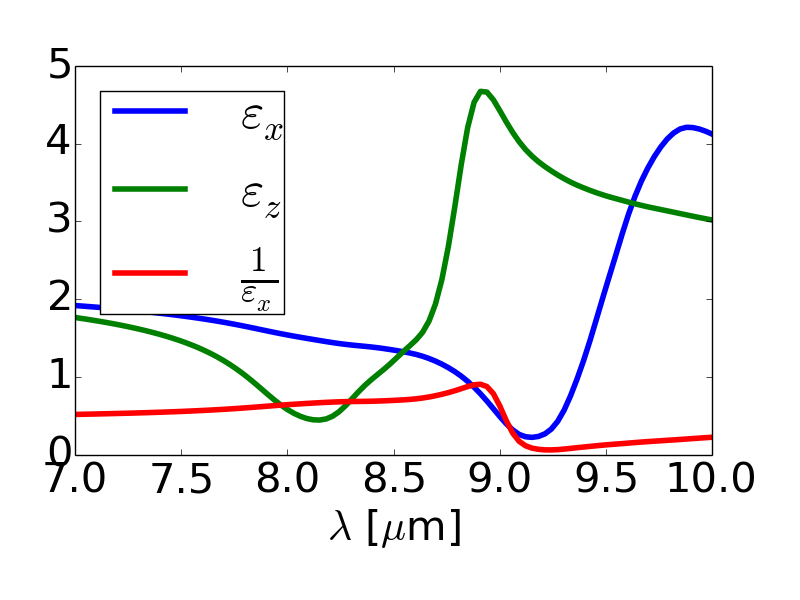
\includegraphics[width=0.6\textwidth]{images/pml/effepsilon-nacl-sio2.png}
	\caption{Współczynniki efektywne wielowarstwy zbudowanej z~$SiO_2$ i~$NaCl$, o~współczynniku wypełnienia przez $SiO_2$ równym $f=0.56$.}
	\label{fig:eff-pml-real}
\end{SCfigure}

Opierając się na zaprojektowanej wielowarstwie można zaproponować jej modyfikację w~geometrii cylindrycznej. W tym przypadku jakość nieodbijającej warstwy absorpcyjnej możemy ocenić na podstawie symulacji, w~których wewnątrz struktury typu \textit{core-shell} zamknięty zostanie walec z~idealnego przewodnika. Rozkład gęstości energii pola E-M dla struktury typu core-shell odpowiadającą rozważanej wielowarstwie, oświetloną falą monochromatyczną dla polaryzacji TM~i~TE przedstawia rysunek \ref{fig:oqecoreshell}.

\begin{figure}[tb]
	\centering
	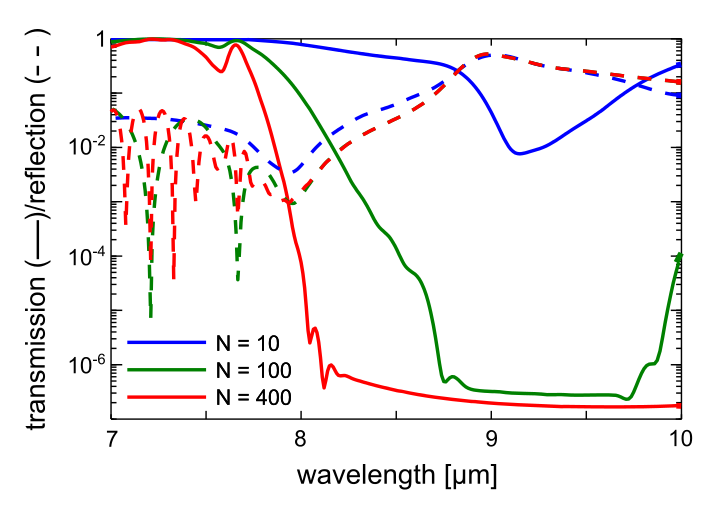
\includegraphics[width=0.6\textwidth]{images/pml/oqe_trans_refl.png}
	\caption{Współczynnik transmisji (linia ciągła) i~odbicia (linia przerywana) dla wielowarstwy złożonej z~$SiO_2$/$NaCl$ zaprojektowanej dla oświetlenia długością fali 8~$\mu$m, dla której współczynniki załamania $n_{\textrm{SiO}_2}=0.41+0.32i$, $n_{\textrm{NaCl}}=$~1.51. Współczynnik wypełnienia struktury przez $SiO_2$ wynosi $f=0.56$, $a=200nm$. Rozważone zostały stosy o~liczbie par warstw $N=$~10,~100 i~400.}
	\label{fig:oqe-trans-refl}
\end{figure}

\begin{figure}[tb]
	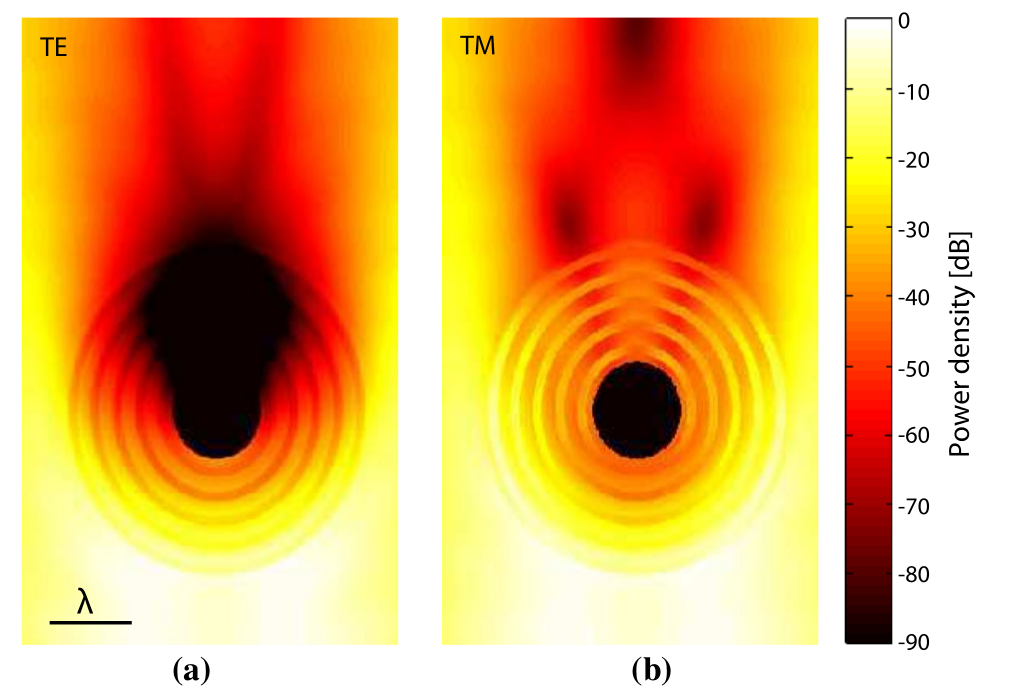
\includegraphics[width=\textwidth]{images/pml/oqe_coreshell.png}
	\caption{Wyniki symulacji w geometrii cylindrycznej dla polaryzacji (a) TE i~(b) TM. Struktura typu core-shell oświetlona jest z~dołu, na rysunku (a) zamieszczono wzorzec długości fali.}
	\label{fig:oqecoreshell}
\end{figure}





Każdy element liniowego układu optycznego możemy wyrazić jako układ filtrujący częstotliwość i częstości przestrzenne oświetlającego ten układ źródła. Poniższy rozdział poświęcony jest modelowaniu propagacji światła przez wielowarstwy metaliczno-dielektryczne wykorzystywane do  budowy elementów optycznych o zaprojektowanych własnościach filtrowania częstości przestrzennych. W przeciwieństwie do przestrzeni swobodnej, będącej przestrzennym filtrem dolnoprzepustowym, mogą one charakteryzować się również transmisją wysokich częstości przestrzennych, które w przestrzeni swobodnej mają charakter fal ewanescentnych. Wykorzystanie układów tego typu umożliwia konstrukcję elementów optycznych działających poza klasycznym ograniczeniem dyfrakcyjnym.

Złamanie ograniczenia dyfrakcyjnego możliwe jest dzięki zastosowaniu materiałów charakteryzujących się ujemnym załamaniem światła, rozumianym jako załamanie pod kątem skierowanym przeciwnie niż wynikałoby to z Prawa Snelliusa. Materiały takie w odniesieniu do tej klasycznej formuły optyki geometrycznej muszą charakteryzować się ujemnym współczynnikiem załamania światła. Korzystając z elektrodynamiki klasycznej opisywanej równaniami Maxwella wiemy, że współczynnik załamania związany jest z przenikalnością elektryczną i magnetyczną ośrodka: $n = \pm \sqrt{ \varepsilon \mu}$. Wybór dodatniej gałęzi pierwiastka jest więc konwencjonalny i musi być dostosowany do sytuacji fizycznej. Ujemna wartość współczynnika załamania światła jest równoważna zmianie kierunku prędkości fazowej, której zwrot jest zgodny ze zwrotem wektora falowego. Pierwszą propozycją definicji ośrodków o ujemnym współczynniku załamania była ujemna wartość iloczynu skalarnego wektora Poyntinga i wektora falowego $\vec{P} \cdot \vec{k} < 0$ podana przez Wiktora Wiesełago \cite{veselago1968electrodynamics}. Ze względu na tę własność materiały takie nazywane są lewoskrętnymi (ang. left-handed) gdyż w stosunku do iloczynu $\vec{E} \times \vec{H}$ nie ma zastosowania reguła prawej dłoni, a przeciwna - lewej.

Materiały lewoskrętne muszą charakteryzować się ujemnymi wartościami $\varepsilon$ i $\mu$ dla tego samego zakresu częstotliwości. Materiały takie nie były do tej pory obserwowane w przyrodzie, eksperymentalnie dowiedziono jednak możliwości sztucznego wytworzenia metamateriałów o takich właściwościach\cite{PhysRevLett.84.4184} przy pomocy SSR(ang split-ring resonator). 

Język używany do opisu działania analizowanych struktur warstwowych wywodzi się z Optyki Fourierowskiej w której podstawowym pojęciem są układy LSI (ang. Linear shift-invariant systems). Opisywane struktury spełniają warunki tego typu układów - nie wykazują własności nieliniowych, oraz są niezmiennicze ze względu na przesunięcia. Wykorzystanie formalizmu Optyki Fourierowskiej umożliwia analityczną ocenę wyników symulacji numerycznych, oraz wprowadza spójny zestaw pojęć wykorzystywanych do opisu rozważanych układów. Dokładniejsze omówienie podstawowych pojęć związanych z układami LSI znajduje się w rozdziale \ref{art:lsi}.



\section{Właściwości dyspersyjne materiałów optycznych w zakresie widzialnym}
Wykorzystywane w~optyce materiały charakteryzują się niską podatnością magnetyczną w~rozważanej części widma, w~związku z~czym przyjmuje się ${\mu(\omega)=1}$. Ze względu na właściwości elektryczne  materiały te możemy  podzielić na dielektryki~i przewodniki. Dielektrykami nazywamy materiały,~w których pod wpływem zewnętrznego pola elektrycznego powstają dipole elektryczne. Powodem powstawania dipoli może być przesunięcie ładunków dodatnich w~stosunku do ujemnych lub powstanie spójnej orientacji przestrzennej dipoli elektrycznych tworzących dany ośrodek. W przeciwieństwie do dielektryków, ze względu na obecność swobodnych nośników ładunku elektrycznego przewodniki nie ulegają polaryzacji w~zewnętrznym polu elektrycznym. W niniejszej pracy jako przewodniki rozważane są metaliczne pierwiastki chemiczne, dlatego terminy przewodnik i~metal traktowane są zamiennie.

\begin{figure}[tb]
	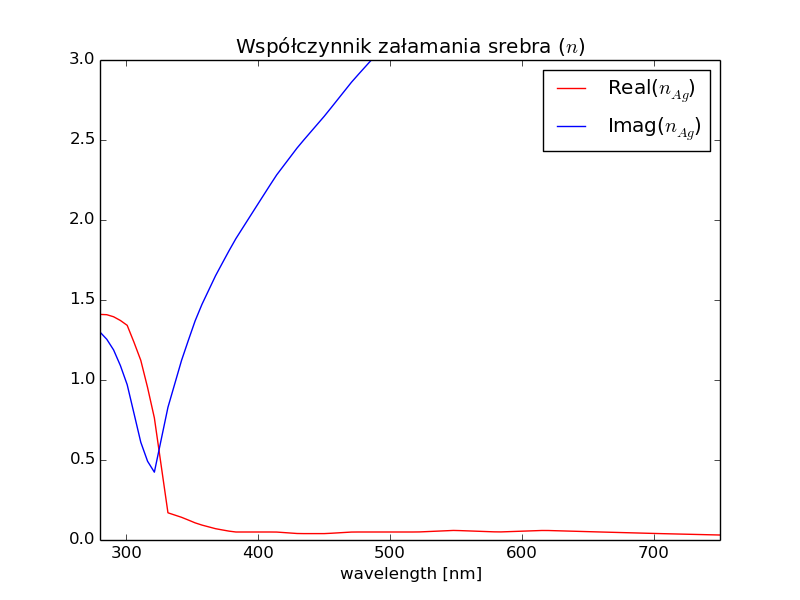
\includegraphics[width=\textwidth]{images/agn.png}
	\caption{Zależność współczynnika załamania od długości fali w~zakresie optycznym dla srebra - $Ag$ \cite{PhysRevB.6.4370}.  }
	\label{fig:agn}
\end{figure}
Zjawiska fizyczne omawiane w~poniższym rozdziale bardzo silnie zależą od przenikalności elektrycznej wykorzystywanych materiałów. W szczególności wymagają wykorzystywania materiałów o~ujemnej przenikalności elektrycznej. Takie własności przejawiają metale, których zastosowanie do nadrozdzielczego obrazowania za pomocą cienkiej warstwy zaproponował John Pendry. Wykorzystanie warstwy znacznie cieńszej od długości fali pozwala na rozprzężenie pola elektrycznego i~magnetycznego przez co możliwe jest nadrozdzielcze obrazowanie za pomocą materiału z~$\mu=$~1\cite{PhysRevLett.85.3966}.

\begin{figure}[tb]
	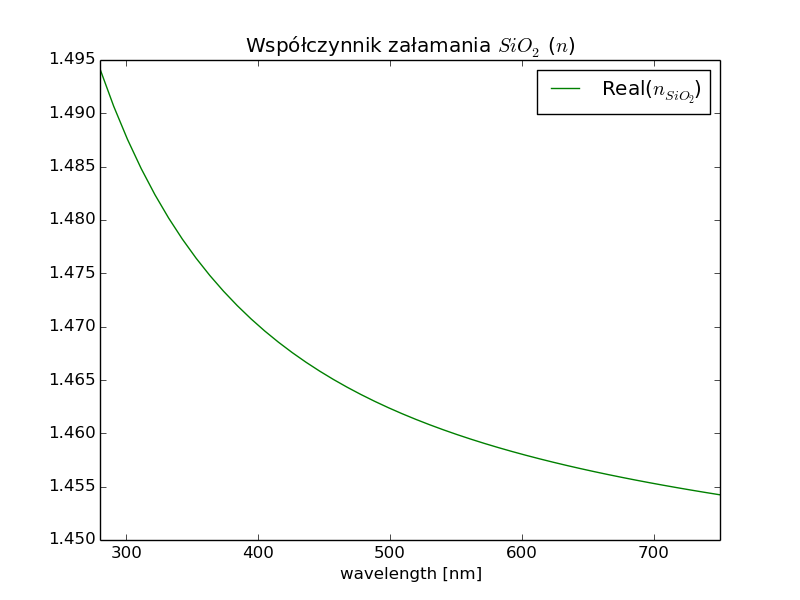
\includegraphics[width=\textwidth]{images/sio2n.png}
	\caption{Zależność współczynnika załamania od długości fali w~zakresie optycznym dla szkła kwarcowego -  $SiO_2$ \cite{MALITSON:65}   }
	\label{fig:sio2n}
\end{figure}
W zakresie optycznym znajdują się częstości rezonansowe atomów metali, co skutkuje silną dyspersją współczynnika załamania i~wysoką absorpcją w~tym zakresie. Zależność rzeczywistej i~urojonej części współczynnika załamania  dla srebra prezentuje wykres \ref{fig:agn}. Na wykresie widać charakterystyczny obszar w~zakresie ok. 310-350~nm, w~którym obserwujemy znaczny spadek części rzeczywistej współczynnika załamania i~minimum zdolności absorpcyjnych. Wysoka wartość części urojonej współczynnika załamania wskazuje na silną absorpcję promieniowania dla długości fali powyżej 350~nm.

Dla dielektryków współczynnik załamania zazwyczaj maleje wraz ze wzrostem długości fali. Zależność ta jest znacznie słabsza niż w~przypadku metali. Jako przykład na wykresie \ref{fig:sio2n} przedstawiono współczynnik załamania $SiO_2$. Urojona część współczynnika załamania dla dielektryków jest mniejsza niż w~przypadku metali. W~szczególność dla przedstawionego szkła kwarcowego w~większości zastosowań jest zaniedbywana.

\begin{figure}[tb]
	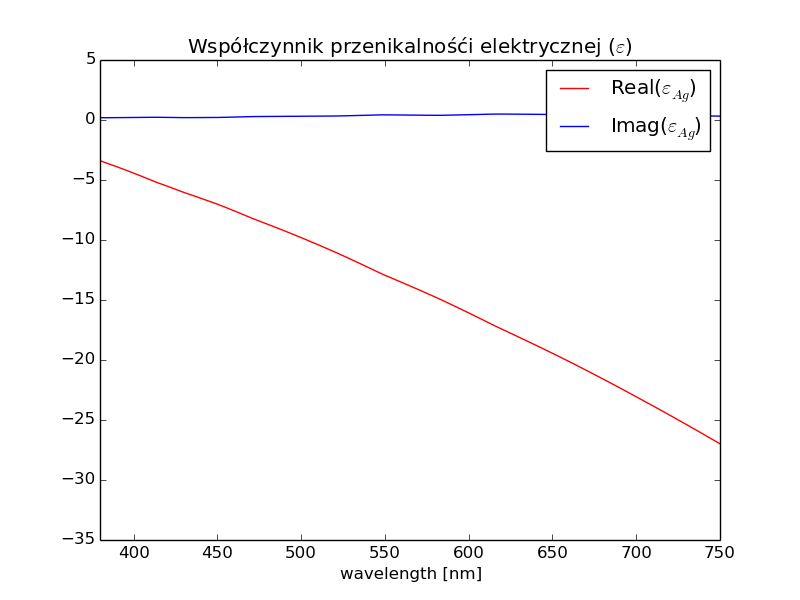
\includegraphics[width=\textwidth]{images/agtio2eps.png}
	\label{fig:agtio2eps}
	\caption{Zależność przenikalności elektrycznej od długości fali w~zakresie optycznym dla srebra $Ag$\cite{PhysRevB.6.4370}. }  
\end{figure}
W celu opisu dyspersyjnych dielektryków z~powodzeniem stosuje się model Lorenza-Lorenza, a~w~niektórych przypadkach wartość $\varepsilon$ bywa traktowana jako stała. W przypadku metali, ze względu na wspomniany charakter rezonansowy $\varepsilon(\omega)$  musi być opisywana przy użyciu modelu Lorenza-Drudego. Dokładniejsze omówienie tego modelu znajduje się w~rozdziale \ref{subart:lorenz-drude}.

Należy zaznaczyć, że pominięty został wpływ wektora falowego na wartości $\varepsilon$ i~µ. W ogólności $\varepsilon(\omega,\vec{k})$ jest funkcją zarówno częstotliwości jak i~wektora falowego, co należy rozumieć jako zależność indukcji elektrycznej $\vec{D}(t,\vec{r})$ nie tylko od historii wzbudzeń poprzedzającej interesujący nas czas $t$, ale również od wzbudzenia fali elektromagnetycznej w~otoczeniu $\vec{r'}$. Ze względu na zależność pola $\vec{D}$ od pola $\vec{E}$ w~otoczeniu, ta klasa zjawisk nazywana jest nielokalnymi. Nie można pomijać wpływu otoczenia na stan polaryzacji $\vec{P}$, gdy zmienność pola elektromagnetycznego jest znacząca na odległościach porównywalnych z~drogą swobodną elektronów w~ośrodku.




\section{Wielowarstwy z bezdyfrkacycyjną propagacja światła}
\begin{figure}[tbh]
	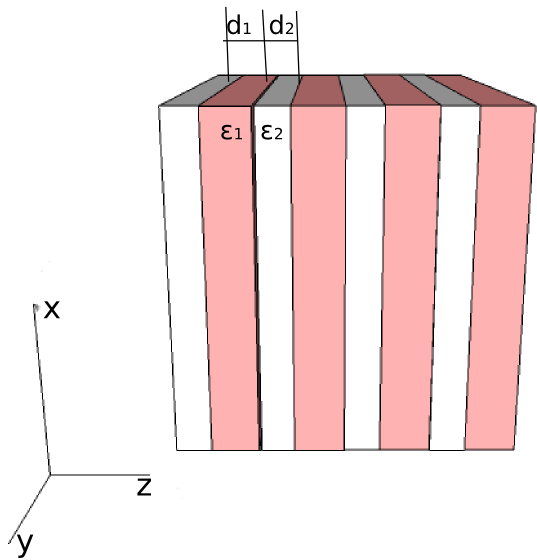
\includegraphics[width=.5\textwidth]{images/multilayer/multilayer-3d.png}
	\caption{Schemat wielowarstwy metaliczno dielektrycznej}
	\label{fig:mulschem}
\end{figure}


Zgodnie z przedstawionymi własnościami materiałowymi obrazowanie z rozdzielczością przekraczającą klasyczne ograniczenie dyfrakcyjne przy pomocy metaliwiąże się z dużymi stratami natężenia światła w wyniku absorbcji. Zwiększenie współczynnika transmisji przez wielowarstwy zawierające metal możliwe jest dzięki wykorzystaniu efektu rezonansowego tunelowania \cite{scalora-transparentmetal}. Chociaż zastosowanie zaproponowane w cytowanej pracy nie było związane z obrazowaniem, to możliwość uzyskania współczynnika transmisji rzędu 70\% dla wielowarstwy zawierającej łącznie 40nm srebra otwiera możliwości wysokiej transmisji i wykorzystania materiałów o ujemnym $\varepsilon$. Schemat wielowarstwy przedstawia rysunek \ref{fig:mulschem}. W proponowanym podejściu obrazowanie nadrozdzielcze nie wynika wprost z zastosowania materiału o $\varepsilon = -1$, ale z efektywnych anizotropowych właściwości powstałęgo w ten sposób  metamateriału \cite{ramakrishna2003imaging}. Przy pomocy przybliżenia ośrodka efektywnego, szerzej omówionego w rozdziale \ref{subart:effmedium}, możemy dobierając grubości warstw do parametrów stosowanych materiałów uzyskać metamateriał o $\varepsilon_z \to \infty$ i $\varepsilon_x \to 0$.


\begin{figure}[tbh]
	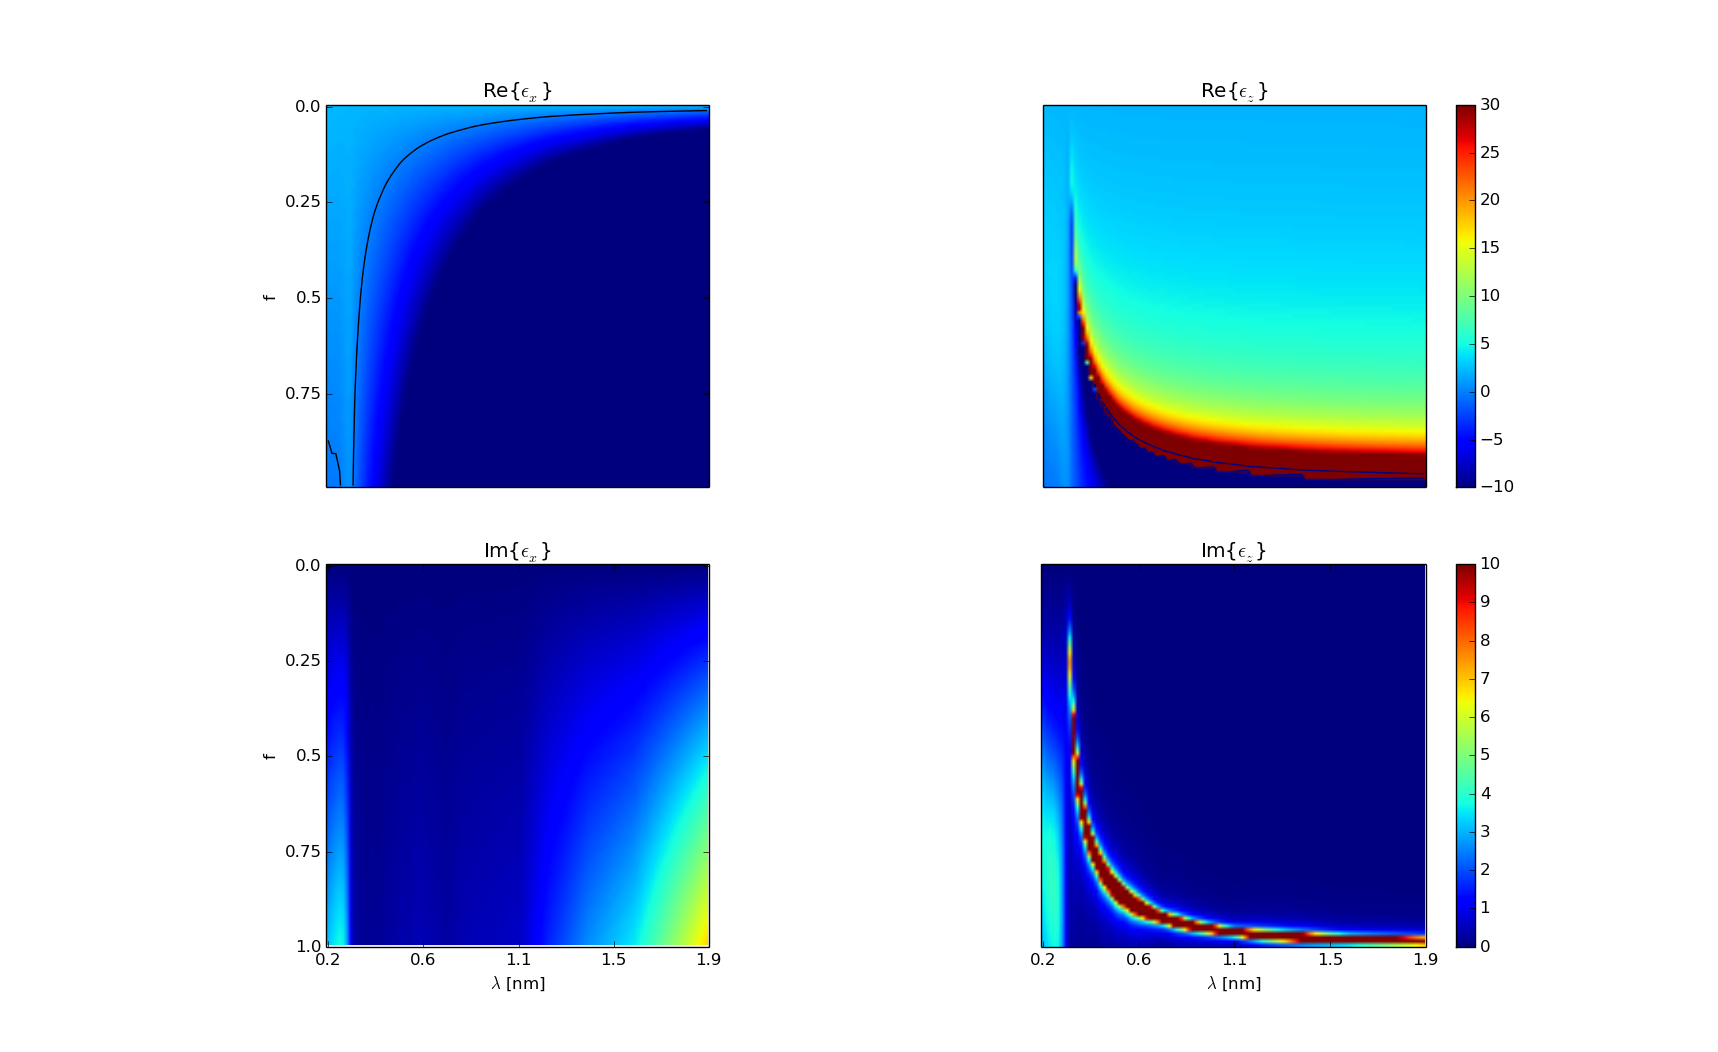
\includegraphics[width=\textwidth]{images/multilayer/agsio2-effective.png}
	\caption{Przenikalność ośrodka efektywnego obliczona zgodnie z \ref{eq:effmedium}  zbudowanego z warstw $Ag$ \cite{PhysRevB.6.4370} i $SiO_2$ \cite{MALITSON:65}. Współczynnik wypełnienia f=1 oznacza, że struktura zbudowana jest jedynie ze srebra. Przy pomocy konturu zaznaczono $\varepsilon_x=0$ oraz $\varepsilon_z=100$.}
	\label{fig:multiex}
%generacja rysuknu:
%./effEpsilon.py database/main/Ag/Johnson.yml database/main/SiO2/Malitson.yml
\end{figure}

Przykład materiałów z których w opisany sposób można konstruować wielowarstwę charateryzującą się transmisją bezdyrakcyjną prezentują wykresy na rysnuknu \ref{fig:multiex}. 






\section{Nadrozdzielczy pryzmat}
Możliwość konstruowania układów warstwowych charakteryzujących się propagacją promieniowania elektromagnetycznego prostopadle do granicy warstw umożliwiła nie tylko konstrukcję supersoczewek, ale również elementów~o bardziej złożonej geometrii. Wykonując ścięcie pod pewnym kątem możemy warstwową supersoczewkę przekształcić~w element optyczny kształtem przypominający pryzmat. Przykład tak powstałego pryzmatu prezentuje rysunek~\ref{fig:prism-schema}. Wykorzystując wielowarstwę~o efektywnych właściwościach zapewniających obrazowanie~z podfalową rozdzielczością, można taki układ wykorzystać do realizacji operacji rzutowania nie podlegającej klasycznemu ograniczeniu dyfrakcyjnemu~\cite{prism2010}. 

Można oczekiwać, że taki element pozwoli uzyskać~ obraz obiekktów o~rozmiarze podfalowym powiększony do rozmiarów umożliwiających obserwację za pomocą tradycyjnych mikroskopów. Możliwe jest również wykorzystanie pryzmatu do zmniejszenia obrazu, dzięki czemu maska o~rozmiarach większych od długości fali może posłużyć do wykonania litografii o~rozmiarach podfalowych.

			\begin{figure}[tbH]
				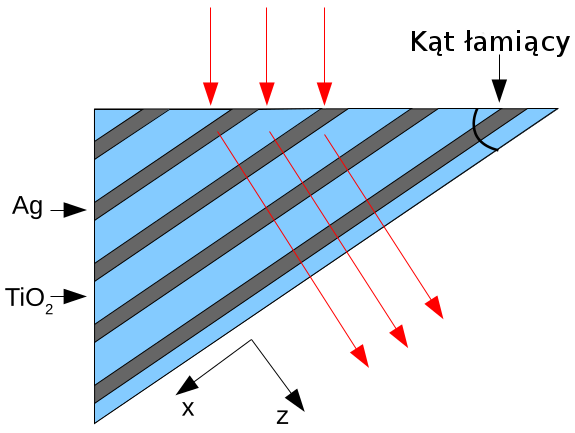
\includegraphics[width=\textwidth]{images/multilayer/prism.png}
				\caption{Schemat pryzmatu zbudowanego z~metamateriału mogącego charakteryzować się kierunkową (prostopadłą do granicy warstw) propagacją fali elektromagnetycznej. Strzałkami schematycznie przedstawiono kierunek propagacji fali E-M.}
				\label{fig:prism-schema}
			\end{figure}


\begin{figure}[btH]
	\centering
			\begin{subfigure}{0.45\textwidth}
				\includegraphics[width=\textwidth]{images/multilayer/prism04.png} \\
				\caption{Kąt łamiący 0.4 rad}
			\end{subfigure}
%			\begin{subfigure}{0.3\textwidth}
%				\includegraphics[width=\textwidth]{images/multilayer/prism08.png} \\
%				\caption{Kąt łamiący 0.8 rad}
%			\end{subfigure}
			\begin{subfigure}{0.45\textwidth}
				\includegraphics[width=\textwidth]{images/multilayer/prism12.png}\\
				\caption{Kąt łamiący 1.2 rad}
			\end{subfigure}
	\caption{Wynik symulacji metodą FDTD propagacji fali E-M przez superpryzmat. Pryzmat oświetlony został wiązką gaussowską o~FWHM $90$~nm i~długości fali $421$~nm~\cite{prism2010}}
\end{figure}

Wykorzystując dwa pryzmaty charakteryzujące się kierunkową propagacją światła, możemy realizować również inne przekształcenia geometryczne na dwuwymiarowych obrazach. Poprzez złożenie dwóch pryzmatów z~rysunku \ref{fig:prism-schema} wzdłuż krawędzi równoległej do osi x, możemy uzyskać element wykonujący na obrazach o~rozmiarach podfalowych operację obrotu. Składając w~ten sposób dwa pryzmaty o~kącie łamiącym równym 45$^\circ$ możemy zrealizować przesunięcie. Wykorzystując trzy pryzmaty możemy połączyć operację rzutowania i~przesunięcia uzyskując efekt powiększenia lub pomniejszenia obrazu w~jednym zintegrowanym mikroelemencie optycznym bez zmiany kierunku propagacji promieniowania E-M~\cite{Zhao:08}.

Ze względu na propagację światła wewnątrz MDM w~określonym kierunku do projektowania układów, których elementy złożone są z~omawianych ściętych wielowarstw metaliczno dielektrycznych wykorzystać można algorytm przypominający śledzenia promieni~(ang. ray tracing). Kierunek promieni w~wiązce wewnątrz wielowarstwy jest wymuszony  przez silnie anizotropową efektywną przenikalność elektryczną wielowarstwy, natomiast w~przestrzeni swobodnej możemy o~nim wnioskować na podstawie klasycznych praw dyfrakcji~\cite{pastuszczak2011slanted}.

\begin{figure}
	\centering
	\begin{subfigure}{.45\textwidth}
		\includegraphics[width=\textwidth]{images/multilayer/prism-ray-tracing1.png}
	\end{subfigure}
	\begin{subfigure}{.45\textwidth}
		\includegraphics[width=\textwidth]{images/multilayer/prism-ray-tracing2.png}
	\end{subfigure}
	\caption{Przykłady algorytmu śledzenia promieni dla wiązki promieni przechodzącej przez pryzmat z~metamateriału umożliwiającego obrazowanie podfalowe~\cite{pastuszczak2011slanted}} 
\end{figure}

%\section{Struktury złożone z kilku wielowarstw}

			\begin{figure}
				\includegraphics[angle=90,width=\textwidth]{images/multilayer/konc_eps_mgr.png}\\
			\end{figure}
			\begin{figure}
				\includegraphics[angle=90,width=\textwidth]{images/multilayer/konc_ene_mgr.png}
			\end{figure}


			\begin{figure}
				\includegraphics[width=\textwidth]{images/multilayer/konc_polk_poynt.png}\\
			\end{figure}


		\begin{figure}
				\includegraphics[width=\textwidth]{images/multilayer/konc_coreshell_energy.png}\\
		\end{figure}

\section{Analiza chropowatosci}
Dotychczas zakładaliśmy, że granice między ośrodkami tworzącymi wielowarstwę są idealnie płaskie. W warunkach eksperymentalnych, przy wykorzystaniu technik umożliwiających naprzemienne układanie kilkunastu warstw różnych materiałów o~grubości od kilkunastu do kilkudziesięciu nanometrów,  takich jak fizyczne osadzanie z~fazy gazowej (ang.~PVD - physical vapour deposition), uzyskanie doskonale gładkich warstw jest niemożliwe. W poniższym rozdziale przeanalizowany zostanie wpływ niedoskonałości warstw na obrazowanie przez struktury MDM(metal-dielektryk-metal).

Podstawowym parametrem wykorzystywanym do opisu chropowatości jest średnia kwadratowa różnic faktycznej grubości warstwy od średniej (ang.~RMS - root mean square), wyrażana wzorem:
\begin{equation}
\textrm{RMS}=\sqrt{\sum_i^n \frac{(x_i -x_0)^2}{n}},
\end{equation}
gdzie $x_i$ są kolejnymi zmierzonymi grubościami, $x_0$ grubością średnią, a $n$ odpowiada liczbie punktów, w~których wykonano pomiar. Różnice uzyskanej w~stosunku do projektowanej grubości warstwy w~blisko położonych punktach nie są zmiennymi losowymi niezależnymi, dlatego do pełnego opisu topologii powierzchni niezbędne jest wykorzystanie funkcji autokorelacji~\cite{stefaniuk2011effect}. Na podstawie pomiarów mikroskopem sił atomowych (ang.~AFM - atomic force microscope) można stwierdzić, że RMS powierzchni podlega statystyce gaussowskiej. Histogram wyników uzyskanych za pomocą pomiarów AFM przedstawia wykres \ref{fig:ag30nm-afmhist}. Dwuwymiarowy skan uzyskany w~pomiarach przedstawia rysunek \ref{fig:ag30nm-afmmeasure}.

\begin{figure}[bt]
		\includegraphics[width=\textwidth]{images/multilayer/ag30nm-afm-measure-hist.png}
		\caption{Histogram odchyleń od średniej grubości dla warstwy $30$~nm napylonej przy pomocy PVD zmierzonych za pomocą AFM} 		\label{fig:ag30nm-afmhist}
\end{figure}

\begin{figure}[bt]
		\includegraphics[width=\textwidth]{images/multilayer/ag30nm-afm-measure.png}
		\caption{Pomiary grubości na powierzchni napylonej warstwy $30$~nm srebra za pomocą AFM. Pomiary wykonał dr~Tomasz~Stefaniuk.} 
		\label{fig:ag30nm-afmmeasure}
\end{figure}


Efektywne współczynniki przenikalności elektrycznej uzyskiwane za pomocą wzoru (\ref{eq:effmedium}) w~znacznym stopniu zmieniają się w~wyniku wprowadzenia chropowatości~\cite{ludwig2012impact}. Szczególnie dużą zmienność można zaobserwować w~okolicach rezonansu dla $\varepsilon_{\perp}$, czyli~w zakresie długości fali, dla którego projektowane są własności metamateriału. Zbliżenie wartości do przewidywanych w~warunkach homogenizacji można zaobserwować w~przypadku struktur, dla których punkty odpowiadające pomiarom grubości z~mikroskopu są bardziej oddalone - próbkowanie pomiaru mikroskopowego jest rzadsze niż w~symulacji numerycznej. Ze względu na przybliżenie granicy warstwy pomiędzy punktami pomiarowymi z~AFM poprzez funkcję gładką, Ludwig i~inni otrzymują większe gładkie obszary na powierzchni symulowanej granicy między ośrodkami~\cite{ludwig2012impact}. 

\begin{figure}[!hbt]
	\begin{center}
	\includegraphics[width=.9\textwidth]{images/multilayer/plp-chropo.png}
	\end{center}
	\caption{Rozkład natężenia pola elektromagnetycznego wewnątrz i~poza strukturą warstwową o~własnościach supersoczewki z~warstwami gładkimi- (a) i (c) oraz chropowatymi- (b) i (d), oświetlonej za pomocą źródła monochromatycznego o~długościach fali odpowiednio (a),(b)~$\lambda=430$~nm  i~(c),(d) $\lambda=490$~nm~\cite{Stolarek_2013}}
	\label{fig:plp-chropo-fdtd}
\end{figure}

Nierówność warstw może mieć pozytywny wpływ na niektóre parametry opisujące zdolności obrazujące wielowarstwy. Uwzględnienie chropowatości może zwiększyć współczynnik transmisji przez granicę dwóch ośrodków poprzez skrócenie zasięgu propagacji plazmonów powierzchniowych w~przypadku przypadkowej chropowatości, oraz dodatkowe wzmocnienie fal ewanescentnych za pomocą sinusoidalnej chropowatości o~okresie podfalowym~\cite{huang2012subwavelength}. Przykład układu dla którego wprowadzenie chropowatości zwiększa współczynnik transmisji dla wąskiego zakresu długości fal, przedstawia rozkład pola elektromagnetycznego na rysunku \ref{fig:plp-chropo-fdtd}~a~-~b. W ogólności jednak wzrost chropowatości powierzchni zmniejsza współczynnik transmisji przez strukturę warstwową, co możemy zaobserwować po zmianie długości fali oświetlającej soczewkę na rozkładach pola na rysunkach \ref{fig:plp-chropo-fdtd}~c~i~d. 

\begin{figure}[bt]
		\includegraphics[width=\textwidth]{images/multilayer/ag30nm-afm-generated.png}
		\caption{Wizualizacja powierzchni chropowatej wygenerowanej na podstawie pomiarów AFM. Generowana dwuwymiarowa macierz losowa podlegające rozkładowi normalnemu o~widmowej gęstości mocy odpowiadającej wynikom pomiarów za pomocą AFM.} 
		\label{fig:ag30nm-afmgene}
%	Generator:
%	pomocnicze/wielowarstw/chropo/gen-chropo.py
\end{figure}


Zmiana właściwości materiałów, z~których zbudowana jest wielowarstwa, na charakteryzujące się mniejszą absorpcją, nie może być wykorzystana do kompensacji strat transmisji w~wyniku nierówności warstw. Wprowadzenie chropowatości prowadzi do powstania losowych zaburzeń rozkładu pola elektromagnetycznego, których interferencja wprowadza zniekształcenie optycznej funkcji przenoszenia~(ang.~OTF - Optical Transfer Function)~\cite{citeulike:2926459}. Odpowiednio dobrany współczynnik absorpcji wewnątrz metali zapewnia szybkie zanikanie losowych zaburzeń umożliwiając zachowanie płaskiego charakteru OTF. Szczególne znaczenie dla zachowania własności obrazowania podfalowego ma płaszczyzna wyjściowa wielowarstwy, na której utrzymanie RMS poniżej $0.6$~nm jest kluczowe dla uzyskania PSF o~szerokości podfalowej~\cite{guo2014negative}.

Należy zwrócić uwagę, że na skutek chropowatości współczynnik $\varepsilon_z$ zostaje zmniejszony w~okolicach rezonansu~\cite{guo2014negative} (dla idealnej supersoczewki $\varepsilon_{z} \to - \infty$), co powoduje, że możliwa jest efektywna transmisja wyższych częstości przestrzennych, a co za tym idzie zwiększenie zdolności rozdzielczej układu. Własności obrazujące, które są optymalne przy płaskim kształcie OTF zostają jednocześnie zaburzone, a ich zachowanie możliwe jest poprzez użycie materiałów o~większym współczynniku absorpcji. Na podstawie takiego rozważania Zhen Guo i~in.~\cite{guo2014negative} wnioskują, że chropowatość w~zasadniczy sposób pogarsza zdolności obrazujące supersoczewki. Zdolność rozdzielcza jest natomiast determinowana poprzez stratność użytych materiałów.

\begin{figure}
	\centering
	\begin{subfigure}[b]{.45\textwidth}
		\includegraphics[width=\textwidth]{images/multilayer/oer-rms01.png}
		\caption{$RMS=0.1$~nm}
	\end{subfigure}
	\begin{subfigure}[b]{.45\textwidth}
		\includegraphics[width=\textwidth]{images/multilayer/oer-rms05.png}
		\caption{$RMS=0.5$~nm}
	\end{subfigure}
	\caption{Wyniki symulacji wielowarstwy o~17 chropowatych granicach ośrodków, z~różnymi wartościami RMS charakteryzującymi chropowatość warstw. Na ilustracji (b) obserwujemy znaczne ograniczenie strumienia fali E-M propagującego się w~pole dalekie na skutek interferencji wielu fal płaskich losowo zaburzonych przez nierówności~\cite{pastuszczak2013engineering}.}
	\label{fig:rmsem}
	
\end{figure}

Porównanie wyników prac numerycznych prowadzonych przez różnych autorów dotyczących wpływu chropowatości na współczynnik transmisji, szerokość i~kształt PSF oraz na zdolność rozdzielczą wielowarstwy wymaga uwzględnienia różnic w~zastosowanej przez nich metodyce. Kluczowym elementem jest sposób generacji powierzchni chropowatej - w~niektórych pracach nie jest uwzględniana autokorelacja nierówności~\cite{guo2014negative} przez co zaniedbane zostają charakterystyczne elementy topologii widoczne w~pomiarach za pomocą AFM. W innych wykorzystywane są algorytmy heurystyczne łączące punkty z~pomiarów mikroskopowych za pomocą wielomianów sklejanych\footnote{tzw. krzywa B-sklejana, w~literaturze polskiej postulowana bywa również nazwa splajn od angielskigo B-spline}~\cite{ludwig2012impact}, w~innych pracach autorzy opierają się na widmowym rozkładzie gęstości mocy zmiennej losowej~\cite{pastuszczak2013engineering}. Przykład powierzchni chropowatej wygenerowanej na podstawie pomiarów z~mikroskopu AFM z~wykorzystaniem ostatniej z~wymienionych metod znajduje się na ilustracji \ref{fig:ag30nm-afmgene}.

Niezależnie od zastosowanej metodyki symulacji pola elektromagnetycznego i~generacji warstw chropowatych składających się na supersoczewki zbudowane ze struktur MDM, wyniki pozwalają na wysunięcie zgodnych wniosków. Uzyskanie nadrozdzielczego obrazowania przez omawiane układy  możliwe jest jest jedynie w~wielowarstwach o~RMS$<1.5$~nm~\citep{guo2014negative,stefaniuk2011effect,ludwig2012impact}. Ponieważ każda chropowata powierzchnia przyczynia się do rozproszenia fali, wraz ze wzrostem liczby warstw własności transmisyjne i~obrazujące stosu MDM stają się bardziej wrażliwe na chropowatości powierzchni \cite{guo2014negative}. W przypadku stosów składających się z~kilkunastu warstw, RMS nawet na poziomie $0.5$~nm może uniemożliwić uzyskanie wysokiego współczynnika transmisji, a co za tym idzie praktycznego wykorzystania tego typu soczewek~\cite{pastuszczak2013engineering}. Wpływ chropowatości na rozkład pola E-M jak i~współczynnik transmisji przez stos metaliczno-dielektryczny prezentują rozkłady pola E-M na rysunku \ref{fig:rmsem}.




%%%%%%%%Obrazki z~publikacji w~PLP - wyniki pomoarow afm w~1d i~2d
%%%%%%%%\begin{figure}
%%%%%%%%		\includegraphics[width=\textwidth]{images/multilayer/plp-afm-chropo-1d.png}\\
%%%%%%%%\end{figure}

%%%%%%%%\begin{figure}
%%%%%%%%		\includegraphics[width=\textwidth]{images/multilayer/plp-afm-chropo.png}\\
%%%%%%%%\end{figure}








\chapter{Podsumowanie}
Wspólnym mianownikiem pracy są wykorzystywane metody oraz podfalowa charakterystyka analizowanych elementów fotonicznych. Warto jednak zwrócić uwagę, że w w poszczególnych rozdziałach analizie poddawane były zupełnie inne zakresy długości fal, charakteryzujące się innymi własnościami materii. Zaczynając od układów do jednokierunkowej transmisji i~skupiania wiązki światła dla zakresu THz~(długości fali ok.~3~cm), które zostały przedstawione w~rozdziale~\ref{chap:thz}, przez struktury warstwowe o~właściwościach UPML w zakresie podczerwieni omówionych w~\ref{roz:pml}, a kończąc w~\ref{art:nondiff} na wielowarstwach metaliczno-dielektrycznych charakteryzujących się bezdyfrakcyjną propagacją promieniowania~E-M dla zakresu widzialnego.

Prace dla zakresu THz koncentrowały się na projektowaniu i~optymalizacji układów, które podlegały późniejszej weryfikacji eksperymentalnej. Wyniki tych prac wskazały na możliwość uzyskania jednokierunkowej transmisji, zgodnej z~twierdzeniem o~wzajemności, w~-1~i~+1 rzędzie dyfrakcyjnym. Przeprowadzona analiza teoretyczna, wraz z potwierdzeniem eksperymentalnym, stanowiły podstawę krytki publikowanych wcześniej prac donoszących o możliwej asymetrii w zerowym rzędzie ugięcia~\cite{Stolarek:13}. W kolejnym kroku zaproponowana została jednokierunkowa soczewka dyfrakcyjna charakteryzująca się kontrastem $C=99.8\%$~\cite{Yavorskiy:14}. 

Dla zakresu THz zaprojektowane zostały również koncentryczne siatki dyfrakcyjne, w których podkład z $GaAs$ można traktować, jako rdzeń falowodu. Konstrukcja ta, pozwoliła na budowę efektywnych anten dla detektorów promieniowania THz, omówionych w~\ref{subart:antenaThz}. Zaprojektowane anteny pozwalają na sprzęganie fal THz z obszarów o rozmiarach kilku centymetrów kwadratowych, z wydajnością  80\%.

W~rozdziale \ref{roz:pml} prowadzone prace realizowane były dla zakresu dalekiej podczerwieni. Przedstawiono prace numeryczne zawierające propozycję realizacji nieodbijającej warstwy pochłaniającej za pomocą układów warstwowych. Całość projektu przedstawia analizę opartą na wyidealizowanych~(nieistniejących fizycznie) materiałach, przez serię przybliżeń, aż do symulacji opartych na własnościach materiałowych zaczerpniętych z~prac eksperymentalnych~\cite{ania2015,stefaniuk2015perfectly}.

W przedostatnim,  rozdziale \ref{art:nondiff}  omówione zostały struktury fotoniczne dla światła widzialnego~(długości fali rzędu kilkuset~nanometrów). Przedstawiono, w~szerokim kontekście literaturowym, wkład autora w~badania dotyczące układów opartych o~wielowarstwy metaliczno-dielektryczne przeznaczone do obrazowania, rzutowania i~koncentracji wiązek promieniowania E-M o~rozmiarach podfalowych. Wykonane symulacje o bardzo dużej rozdzielczości pozwoliły określić wymagania na parametry statystyczne opisujące gładkość napylonych warstw umożliwiającą eksperymentalną weryfikację obrazowania podfalowego.

Ze względu na duże wymogi mocy obliczeniowej jak i złożoność pamięciową wykorzystywanych metod, konieczne było wykorzystanie infrastruktury HPC~(ang. High-performance computing). Używane zasoby obliczeniowe były udostępniane przez Interdyscyplinarne Centrum Modelowania Matematycznego i~Komputerowego UW oraz infrastrukturę PLgrid. 




\printnomenclature

\addcontentsline{toc}{chapter}{Bibliografia}
%\bibliographystyle{abbrvnat}
\bibliographystyle{osa}
\bibliography{bibliografia}

\addcontentsline{toc}{chapter}{Spis ilustracji}
\listoffigures
\addcontentsline{toc}{chapter}{Skorowidz skrótowców}
\chapter*{Skorowidz skrótowców}
\noindent ABC - ang. absorbing boundary condition, absorbujący warunek brzegowy
\\AFM - ang. atomic force microscope, mikroskop sił atomowych
\\BOR FDTD - ang. body of revolution FDTD, nazwa algorytmu FDTD służącego do prowadzenia symulacji dla struktur o symetrii cylindrycznej 
\\BPM - ang. beam propagation method, metoda propagacji wiązki
\\DMG - and. double metallic grating, podwójna metalowa siatka dyfrakcyjna
\\EMA - ang. effective medium approximation, przybliżenie ośrodka efektywnego
\\EMT - ang. effective medium theory, teoria ośrodka efektywnego
\\FDTD - ang. finite difference time domain, metoda różnic skończonych w dziedzinie czasu
\\FEM - ang. finite-element method, metoda elementu skończonego
\\FWHM - ang. full width at half maximum, szerokość połówkowa
\\HPC - ang. high performance computing, obliczenia z wykorzystaniem komputerów dużej mocy
\\LSI - ang linear shift-invariant, liniowy niezmienniczy ze względu na przesunięcia
\\OTF - ang. optical transfer function, optyczna funkcja przenoszenia
\\PEC - ang. perfect electric conductor, doskonały przewodnik
\\PMC - ang. perfect magnetic conductor, doskonały przewodnik magnetyczny 
\\PML - ang. perfectly matched layer, warstwa na granicy z którą nie występuje zjawisko odbicia
\\PSF - ang. point spread function, funkcja rozmycia punktu
\\PTFE - politetrafluoroetylen, teflon
\\PVD - ang. physical vapour deposition, fizycznie osadzenie z fazy gazowej
\\RAM - ang. random access memory, pamięć o dostępie swobodnym
\\RCWA - ang. rigorous coupled wave analysis, półanalityczna metoda obliczeniowa implementowana w przestrzeni fourierowskiej
\\RMS - ang. root mean square, średnia kwadratowa
\\SMG - ang. single metallic grating, pojedyncza siatka metalowa - termin stosowany dla podkreślenia różnicy w stosunku do DMG
\\SMM - ang. scattering matrix method, metoda obliczeniowa wykorzystująca tzw. macierze rozpraszania
\\SNR - ang. signal to noise ratio, stosunek sygnału do szumu
\\SP - ang. surface plasmon, plazmon powierzchniowy
\\SPP - ang. surface plasmon polariton, powierzchniowy plazmon-polaryton
\\SRR - ang. split-ring resonator, popularny układ wykorzystywany do projektowania metamateriałów dla fal elektromagnetycznych z zakresu mikrofalowego
\\TE - ang. transverse electric, określenie polaryzacji fali elektromagnetycznej, w~której pole elektryczne drga równolegle do rozważanej płaszczyzny
\\TFSF - ang. total field scattered field, rodzaj źródła, w którym nieodbijające warunki brzegowe są uzyskiwane poprzez podział całości obszaru symulacji na pola całkowite i rozproszone
\\TM - ang. transverse magnetic, określenie polaryzacji fali elektromagnetycznej, w~której pole magnetyczne drga równolegle do rozważanej płaszczyzny
\\TMM - ang. transfer matrix method, metoda obliczeniowa wykorzystująca macierze przejścia
\\UPML - ang.  uniaxial perfectly matched layer, materiał typu PML realizowany za pomocą ośrodka anizotropowego
\\UW - Uniwersytet Warszawski

\end{document}
